% !TeX encoding = UTF-8
% !TeX program = xelatex
% !TeX spellcheck = en_US

\documentclass[degree=bachelor, fontset=windows]{thuthesis}
  % 学位 degree:
  %   doctor | master | bachelor | postdoc
  % 学位类型 degree-type:
  %   academic(默认)| professional
  % 语言 language
  %   chinese(默认)| english
  % 字体库 fontset
  %   windows | mac | fandol | ubuntu
  % 建议终版使用 Windows 平台的字体编译


% 论文基本配置,加载宏包等全局配置
% !TeX root = ./thuthesis-example.tex

% 论文基本信息配置

\thusetup{
  %******************************
  % 注意:
  %   1. 配置里面不要出现空行
  %   2. 不需要的配置信息可以删除
  %   3. 建议先阅读文档中所有关于选项的说明
  %******************************
  %
  % 输出格式
  %   选择打印版(print)或用于提交的电子版(electronic),前者会插入空白页以便直接双面打印
  %
  output = print,
  %
  % 标题
  %   可使用“\\”命令手动控制换行
  %
  title  = {出租车调度系统中的树状区块链的跨链操作的设计研究},
  title* = {Design and Research on Cross chain Operations of Tree Blockchain in Taxi Dispatching System},
  %
  % 学科门类
  %   1. 学术型
  %      - 中文
  %        需注明所属的学科门类,例如:
  %        哲学、经济学、法学、教育学、文学、历史学、理学、工学、农学、医学、
  %        军事学、管理学、艺术学
  %      - 英文
  %        博士:Doctor of Philosophy
  %        硕士:
  %          哲学、文学、历史学、法学、教育学、艺术学门类,公共管理学科
  %          填写“Master of Arts“,其它填写“Master of Science”
  %   2. 专业型
  %      直接填写专业学位的名称,例如:
  %      教育博士、工程硕士等
  %      Doctor of Education, Master of Engineering
  %   3. 本科生不需要填写
  %
%  degree-category  = {工学硕士},
%  degree-category* = {Master of Science},
  %
  % 培养单位
  %   填写所属院系的全名
  %
  department = {新雅书院/计算机科学与技术系},
  %
  % 学科
  %   1. 研究生学术型学位,获得一级学科授权的学科填写一级学科名称,其他填写二级学科名称
  %   2. 本科生填写专业名称,第二学位论文需标注“(第二学位)”
  %
  discipline  = {计算机科学与技术},
  discipline* = {Computer Science and Technology},
  %
  % 专业领域
  %   1. 设置专业领域的专业学位类别,填写相应专业领域名称
  %   2. 2019 级及之前工程硕士学位论文,在 `engineering-field` 填写相应工程领域名称
  %   3. 其他专业学位类别的学位论文无需此信息
  %
  % professional-field  = {计算机技术},
  % professional-field* = {Computer Technology},
  %
  % 姓名
  %
  author  = {狄永正},
  author* = {Di Yongzheng},
  %
  % 指导教师
  %   中文姓名和职称之间以英文逗号“,”分开,下同
  %
  supervisor  = {向勇, 副研究员},
  supervisor* = {associate professor Xiang Yong},
  %
  % 副指导教师
  %
  %associate-supervisor  = {陈文光, 教授},
  %associate-supervisor* = {Professor Chen Wenguang},
  %
  % 联合指导教师
  %
  % co-supervisor  = {某某某, 教授},
  % co-supervisor* = {Professor Mou Moumou},
  %
  % 日期
  %   使用 ISO 格式;默认为当前时间
  %
  % date = {2019-07-07},
  %
  % 是否在中文封面后的空白页生成书脊(默认 false)
  %
  include-spine = false,
  %
  % 密级和年限
  %   秘密, 机密, 绝密
  %
  % secret-level = {秘密},
  % secret-year  = {10},
  %
  % 博士后专有部分
  %
  % clc                = {分类号},
  % udc                = {UDC},
  % id                 = {编号},
  % discipline-level-1 = {计算机科学与技术},  % 流动站(一级学科)名称
  % discipline-level-2 = {系统结构},          % 专业(二级学科)名称
  % start-date         = {2011-07-01},        % 研究工作起始时间
}

% 载入所需的宏包

% 定理类环境宏包
\usepackage{amsthm}
% 也可以使用 ntheorem
% \usepackage[amsmath,thmmarks,hyperref]{ntheorem}

\thusetup{
  %
  % 数学字体
  % math-style = GB,  % GB | ISO | TeX
  math-font  = xits,  % stix | xits | libertinus
}

% 可以使用 nomencl 生成符号和缩略语说明
% \usepackage{nomencl}
% \makenomenclature

% 表格加脚注
\usepackage{threeparttable}

% 表格中支持跨行
\usepackage{multirow}

% 固定宽度的表格。
% \usepackage{tabularx}

% 跨页表格
\usepackage{longtable}

% 算法
\usepackage{algorithm}
\usepackage{algorithmic}

% 量和单位
\usepackage{siunitx}

% 参考文献使用 BibTeX + natbib 宏包
% 顺序编码制
\usepackage[sort]{natbib}
\bibliographystyle{thuthesis-numeric}

% 著者-出版年制
% \usepackage{natbib}
% \bibliographystyle{thuthesis-author-year}

% 本科生参考文献的著录格式
% \usepackage[sort]{natbib}
% \bibliographystyle{thuthesis-bachelor}

% 参考文献使用 BibLaTeX 宏包
% \usepackage[style=thuthesis-numeric]{biblatex}
% \usepackage[style=thuthesis-author-year]{biblatex}
% \usepackage[style=apa]{biblatex}
% \usepackage[style=mla-new]{biblatex}
% 声明 BibLaTeX 的数据库
% \addbibresource{ref/refs.bib}

% 定义所有的图片文件在 figures 子目录下
\graphicspath{{figures/}}

% 数学命令
\makeatletter
\newcommand\dif{%  % 微分符号
  \mathop{}\!%
  \ifthu@math@style@TeX
    d%
  \else
    \mathrm{d}%
  \fi
}
\makeatother

% hyperref 宏包在最后调用
\usepackage{hyperref}



\begin{document}

% 封面
\maketitle

% 学位论文指导小组、公开评阅人和答辩委员会名单
% 本科生不需要
% !TeX root = ../thuthesis-example.tex

\begin{committee}[name={学位论文指导小组、公开评阅人和答辩委员会名单}]

  \newcolumntype{C}[1]{@{}>{\centering\arraybackslash}p{#1}}

  \section*{指导小组名单}

  \begin{center}
    \begin{tabular}{C{3cm}C{3cm}C{9cm}@{}}
      李XX & 教授     & 清华大学 \\
      王XX & 副教授   & 清华大学 \\
      张XX & 助理教授 & 清华大学 \\
    \end{tabular}
  \end{center}


  \section*{公开评阅人名单}

  \begin{center}
    \begin{tabular}{C{3cm}C{3cm}C{9cm}@{}}
      刘XX & 教授   & 清华大学                    \\
      陈XX & 副教授 & XXXX大学                    \\
      杨XX & 研究员 & 中国XXXX科学院XXXXXXX研究所 \\
    \end{tabular}
  \end{center}


  \section*{答辩委员会名单}

  \begin{center}
    \begin{tabular}{C{2.75cm}C{2.98cm}C{4.63cm}C{4.63cm}@{}}
      主席 & 赵XX                  & 教授                    & 清华大学       \\
      委员 & 刘XX                  & 教授                    & 清华大学       \\
          & \multirow{2}{*}{杨XX} & \multirow{2}{*}{研究员} & 中国XXXX科学院 \\
          &                       &                         & XXXXXXX研究所  \\
          & 黄XX                  & 教授                    & XXXX大学       \\
          & 周XX                  & 副教授                  & XXXX大学       \\
      秘书 & 吴XX                  & 助理研究员              & 清华大学       \\
    \end{tabular}
  \end{center}

\end{committee}



% 也可以导入 Word 版转的 PDF 文件
% \begin{committee}[file=figures/committee.pdf]
% \end{committee}


% 使用授权的说明
% \copyrightpage
% 将签字扫描后授权文件 scan-copyright.pdf 替换原始页面
\copyrightpage[file=scan-copyright.pdf]

\frontmatter
% !TeX root = ../thuthesis-example.tex

% 中英文摘要和关键字

\begin{abstract}
随着科技的进步,汽车行业的快速发展和广泛应用,车辆之间的交互将变得必不可少。为了创建一个更加安全高效的交通环境,区块链技术已经被应用于车联网中。区块链的去中心化、独立性等特点使得在出租车调度系统中应用区块链技术能够消除中介,允许乘客与司机的直接交流与交易,在网络出租车服务中使用区块链有助于参与的所有利益相关方关系更加紧密。

然而传统的区块链是单链结构,在处理大量交易时,会导致链条过长,从而消耗大量时间和能量,进而执行效率低下。为解决该问题,我们在出租车调度系统中应用“树状区块链”。树状区块链根据地理位置的Geohash编码划分子链,形成分支区块管理其下子链,不同子链管理不同区域的这样一种树状字典树结构。

本文首先是阅读了树状区块链的部分实现源码,对于一些源码核心功能函数给出了注释说明,之后,基于现有项目结构完成了对树状区块链应用于出租车调度系统的复现工作,并验证多子链并行运行的负载性能。此外,本文还验证了树状区块链的跨子链资产转移功能的正确性,并测试了其性能。在以上工作的基础之上,本文尝试对现有出租车调度系统的跨区域(跨子链)交易进行改进。现有的出租车调度系统仅支持一个子链内部的交易,但在实际应用场景中,乘客与车辆分处不同区域(不同子链)的概率非常大,针对这样的现实情况,本文尝试对现有的出租车调度系统进行改进使其支持跨链的交易操作,设计并实现了跨区域交易的相关测试以及跨区域交易的合约,最终给出了一个简易的能够实现跨链交易的调度过程,设计实验验证了实现的正确性。

  % 关键词用“英文逗号”分隔,输出时会自动处理为正确的分隔符
  \thusetup{
    keywords = {区块链, 车联网, 树状区块链跨子链},
  }
\end{abstract}

\begin{abstract*}
    With the rapid development and widespread application of technology in the automotive industry, the interaction between vehicles will become essential. In order to create a safer and more efficient transportation environment, it is proposed to apply blockchain technology to the Internet of Vehicles. The decentralization and independence of blockchain technology can eliminate intermediaries in taxi dispatch systems. This allows for direct communication and transactions between passengers and drivers, and the use of blockchain technology in online taxi services can help to strengthen relationships between all stakeholders involved.
    
    However, traditional blockchain technology is characterized by a single chain structure, which results in a long chain and consumes significant time and energy when processing a large number of transactions. In this situation, it has poor execution efficiency. To address this issue, we implement a "tree-structured blockchain" in the taxi dispatch system. The tree-structured blockchain divides the sub-chains based on Geohash encoding of geographical locations, forming branching blocks to manage the sub-chains. This creates a tree-structured trie structure in which different sub-chains manage different areas.
    
    This thesis begins by reading some of the source code for tree-structured blockchains and providing annotations for certain core functions. Following this, the article reproduces the use of tree-structured blockchains in a taxi dispatch system based on the existing project structure, and verifies the load performance of parallel running of multiple sub-chains. In addition, the article verifies the correctness of cross-sub-chain asset transfer in tree-structured blockchains and tests its performance. Building on this work, the article attempts to improve existing taxi dispatch systems by enabling cross-regional (cross-sub-chain) transactions. Current taxi dispatch systems only support transactions within a single sub-chain, but in real-world scenarios, the likelihood of passengers and vehicles being located in different areas (different sub-chains) is high. To address this, the author attempts to enable cross-chain transactions in existing taxi dispatch systems by designing and implementing tests and contracts for cross-regional transactions, ultimately providing a simple process for enabling cross-chain transactions and verifying its correctness through experimentation.

  % Use comma as separator when inputting
  \thusetup{
    keywords* = {Blockchain, Internet of Vehicles, Tree-structured Blockchain Cross-Subchain},
  }
\end{abstract*}

% 目录
\tableofcontents

% 符号对照表
% % !TeX root = ../thuthesis-example.tex

\begin{denotation}[3cm]
  \item[PI] 聚酰亚胺
  \item[MPI] 聚酰亚胺模型化合物,N-苯基邻苯酰亚胺
  \item[PBI] 聚苯并咪唑
  \item[MPBI] 聚苯并咪唑模型化合物,N-苯基苯并咪唑
  \item[PY] 聚吡咙
  \item[PMDA-BDA] 均苯四酸二酐与联苯四胺合成的聚吡咙薄膜
  \item[MPY] 聚吡咙模型化合物
  \item[As-PPT] 聚苯基不对称三嗪
  \item[MAsPPT] 聚苯基不对称三嗪单模型化合物,3,5,6-三苯基-1,2,4-三嗪
  \item[DMAsPPT] 聚苯基不对称三嗪双模型化合物(水解实验模型化合物)
  \item[S-PPT] 聚苯基对称三嗪
  \item[MSPPT] 聚苯基对称三嗪模型化合物,2,4,6-三苯基-1,3,5-三嗪
  \item[PPQ] 聚苯基喹噁啉
  \item[MPPQ] 聚苯基喹噁啉模型化合物,3,4-二苯基苯并二嗪
  \item[HMPI] 聚酰亚胺模型化合物的质子化产物
  \item[HMPY] 聚吡咙模型化合物的质子化产物
  \item[HMPBI] 聚苯并咪唑模型化合物的质子化产物
  \item[HMAsPPT] 聚苯基不对称三嗪模型化合物的质子化产物
  \item[HMSPPT] 聚苯基对称三嗪模型化合物的质子化产物
  \item[HMPPQ] 聚苯基喹噁啉模型化合物的质子化产物
  \item[PDT] 热分解温度
  \item[HPLC] 高效液相色谱(High Performance Liquid Chromatography)
  \item[HPCE] 高效毛细管电泳色谱(High Performance Capillary lectrophoresis)
  \item[LC-MS] 液相色谱-质谱联用(Liquid chromatography-Mass Spectrum)
  \item[TIC] 总离子浓度(Total Ion Content)
  \item[\textit{ab initio}] 基于第一原理的量子化学计算方法,常称从头算法
  \item[DFT] 密度泛函理论(Density Functional Theory)
  \item[$E_a$] 化学反应的活化能(Activation Energy)
  \item[ZPE] 零点振动能(Zero Vibration Energy)
  \item[PES] 势能面(Potential Energy Surface)
  \item[TS] 过渡态(Transition State)
  \item[TST] 过渡态理论(Transition State Theory)
  \item[$\increment G^\neq$] 活化自由能(Activation Free Energy)
  \item[$\kappa$] 传输系数(Transmission Coefficient)
  \item[IRC] 内禀反应坐标(Intrinsic Reaction Coordinates)
  \item[$\nu_i$] 虚频(Imaginary Frequency)
  \item[ONIOM] 分层算法(Our own N-layered Integrated molecular Orbital and molecular Mechanics)
  \item[SCF] 自洽场(Self-Consistent Field)
  \item[SCRF] 自洽反应场(Self-Consistent Reaction Field)
\end{denotation}



% 也可以使用 nomencl 宏包,需要在导言区
% \usepackage{nomencl}
% \makenomenclature

% 在这里输出符号说明
% \printnomenclature[3cm]

% 在正文中的任意为都可以标题
% \nomenclature{PI}{聚酰亚胺}
% \nomenclature{MPI}{聚酰亚胺模型化合物,N-苯基邻苯酰亚胺}
% \nomenclature{PBI}{聚苯并咪唑}
% \nomenclature{MPBI}{聚苯并咪唑模型化合物,N-苯基苯并咪唑}
% \nomenclature{PY}{聚吡咙}
% \nomenclature{PMDA-BDA}{均苯四酸二酐与联苯四胺合成的聚吡咙薄膜}
% \nomenclature{MPY}{聚吡咙模型化合物}
% \nomenclature{As-PPT}{聚苯基不对称三嗪}
% \nomenclature{MAsPPT}{聚苯基不对称三嗪单模型化合物,3,5,6-三苯基-1,2,4-三嗪}
% \nomenclature{DMAsPPT}{聚苯基不对称三嗪双模型化合物(水解实验模型化合物)}
% \nomenclature{S-PPT}{聚苯基对称三嗪}
% \nomenclature{MSPPT}{聚苯基对称三嗪模型化合物,2,4,6-三苯基-1,3,5-三嗪}
% \nomenclature{PPQ}{聚苯基喹噁啉}
% \nomenclature{MPPQ}{聚苯基喹噁啉模型化合物,3,4-二苯基苯并二嗪}
% \nomenclature{HMPI}{聚酰亚胺模型化合物的质子化产物}
% \nomenclature{HMPY}{聚吡咙模型化合物的质子化产物}
% \nomenclature{HMPBI}{聚苯并咪唑模型化合物的质子化产物}
% \nomenclature{HMAsPPT}{聚苯基不对称三嗪模型化合物的质子化产物}
% \nomenclature{HMSPPT}{聚苯基对称三嗪模型化合物的质子化产物}
% \nomenclature{HMPPQ}{聚苯基喹噁啉模型化合物的质子化产物}
% \nomenclature{PDT}{热分解温度}
% \nomenclature{HPLC}{高效液相色谱(High Performance Liquid Chromatography)}
% \nomenclature{HPCE}{高效毛细管电泳色谱(High Performance Capillary lectrophoresis)}
% \nomenclature{LC-MS}{液相色谱-质谱联用(Liquid chromatography-Mass Spectrum)}
% \nomenclature{TIC}{总离子浓度(Total Ion Content)}
% \nomenclature{\textit{ab initio}}{基于第一原理的量子化学计算方法,常称从头算法}
% \nomenclature{DFT}{密度泛函理论(Density Functional Theory)}
% \nomenclature{$E_a$}{化学反应的活化能(Activation Energy)}
% \nomenclature{ZPE}{零点振动能(Zero Vibration Energy)}
% \nomenclature{PES}{势能面(Potential Energy Surface)}
% \nomenclature{TS}{过渡态(Transition State)}
% \nomenclature{TST}{过渡态理论(Transition State Theory)}
% \nomenclature{$\increment G^\neq$}{活化自由能(Activation Free Energy)}
% \nomenclature{$\kappa$}{传输系数(Transmission Coefficient)}
% \nomenclature{IRC}{内禀反应坐标(Intrinsic Reaction Coordinates)}
% \nomenclature{$\nu_i$}{虚频(Imaginary Frequency)}
% \nomenclature{ONIOM}{分层算法(Our own N-layered Integrated molecular Orbital and molecular Mechanics)}
% \nomenclature{SCF}{自洽场(Self-Consistent Field)}
% \nomenclature{SCRF}{自洽反应场(Self-Consistent Reaction Field)}


% 正文部分
\mainmatter
% !TeX root = ../thuthesis-example.tex

\chapter{绪论}

\section{研究背景}

随着时代的发展,现阶段,随着城市里的流动车辆数量的不断攀升,给城市的交通带来的负担也日益沉重。根据最新的数据,目前我国的汽车总数已经突破3亿辆,近年来的年均增长率超过2000万辆,而且,每千户家庭的汽车数也已经突破225辆,平均到每百户当中便有60辆汽车。 在当下社会中,人们都过着快节奏的生活,对交通的便捷性需求自然日益增长。越来越多的人会选择出租车或网约车出行;出租车,网约车有着针对性强,更为便捷,流动基数更多等特点,也切实的便捷了人们的出行 。

车联网技术属于物联网技术的范畴,是互联网、电子、汽车等产业融合创新的产物,其旨在通过实现车辆之间的相互通信,最终构建安全高效智能的交通体系 。为了确保车联网的高度稳定,我们必须采取措施来确保它的安全。对此,区块链所具有的去中心化、时序数据、集体维护、可编程和安全可信的特点,使得人们相信其可有效服务于车联网的应用当中 。将区块链技术应用于车联网中,使用区块链技术来构建车辆与路测节点间的特殊自组网,进行车辆间或车辆与路侧节点间的数据交互。通过采取区块链技术,我们能够在车联网中实现更加透明、安全的交易,从而消除中央控制,构建一个更加可信任、无需中央控制的数字资产,从而实现共享经济的发展 。

在出租车调度系统中应用该技术可以消除中介,允许乘客与司机的直接交流与交易,能够为双方提供更为可信的验证,降低信任成本。在网络出租车服务中使用区块链技术有助于参与的所有利益相关方关系更加紧密 。

\section{相关技术调研}

\subsection{区块链概述}

在2008年,一位自称中本聪的人提出了区块链技术 (Blockchain technology,简称BT)。通过使用区块链技术,我们可以建立一个完整、可追溯、可扩展、可信任的网络。区块链利用块链式的数据结构来验证与存储数据,其通过使用共识算法、加密算法、智能合约编程等技术,实现对数据进行安全的访存、传输以及维护,从而实现对信息的有效管理,是一种全新的分布式基础架构与计算范式 。

区块链可以创建无法篡改且端到端加密的记录,用区块链技术所串接的分布式账本能让两方有效纪录交易,且可永久查验此交易,有助于防止欺诈和未经授权的活动。此外,区块链有更大的透明度:由于区块链使用分布式账本,导致交易和数据在多个位置采取完全相同的方式进行记录。区块链技术的核心优势在于它的去中心化特性,即所有拥有访问权限的网络参与者都可以共享相同的信息,从而保证了信息的完全透明度。此外,它的去中心化特性使得每个节点都可以独立地操作,无需受到任何外部干扰,从而提升了系统的可靠性和安全性 。


\subsection{区域索引的树状区块链}

将传统的区块链应用到出租车调度系统中的一个很大的弊端是,传统区块链在面对数量庞大的节点时,因为节点全在一条链上,其查询效率必然会降低;此外,传统区块链结构不能很好地支持对发生在特定区域的事务的查询:用户需要回溯链结构上的所有事务,然后匹配交易发生的位置  。为满足车联网所需的性能要求,大幅度提高地理区块链的区域搜索速度,项目决定用“树状区块链”来代替传统区块链。

在实现树状区块链之前,首先实现了支持区域索引的区块链,该区块链可以基于地理位置信息索引到对应的交易 。之后,在区域索引区块链的基础上,实验室逐步完成了现有的支持区域索引的树状区块链。

如图\ref{fig:树状区块链示意图}所示,树状区块链按照Geohash编码方式划分树状结构,根据不同长度的Geohash编码表示父链与子链关系,文献 说明以Geohash为基础的空间索引算法具有对海量地理数据的高性能查询能力。不同于传统区块链的结构单一,树状区块链结构中的区块根据其作用不同可以划分为创世块(Genesis Block),分支区块(Branch Block)和普通区块(Common Block)三类。

\begin{itemize}
    \item 其中创世块是所有区块的根节点,所有的区块链都有相同的创世块Gensis,然后根据Geohash范围划分不同的区域子链。
    \item 分支区块以Geohash作为索引,是指定分支的第一个区块,只维护直接下层区域的索引信息,不记录交易信息。分支区块由于具备指向同层级前一个分支区块的平行链指针使得原有单链结构成为树状多链构。
    \item 普通区块则基本与传统区块相同。
\end{itemize}

\begin{figure}
	\centering
	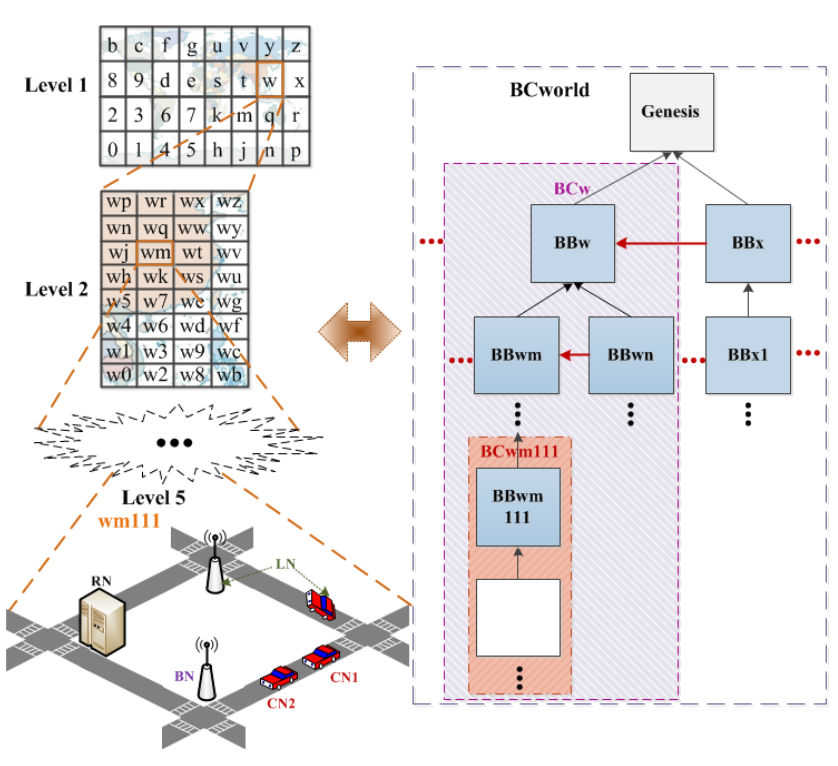
\includegraphics[width=\textwidth]{figures/树状区块链示意图.png}
	\caption{树状区块链示意图}
	\label{fig:树状区块链示意图}
\end{figure}

图\ref{fig:树状区块链内部结构属性示意图}中是树状区块链的内部结构属性示意图,展示了区块链的存储的各种属性,以太坊的结构包括三种查找树:收据查找树、地理状态查找树和交易查找树。除此之外,还添加了一个区域状态查找树来快速查询与分层地理位置相关的数据,以及一个帐户位置查找树来支持查询每辆车的历史交易位置。

\begin{figure}
	\centering
	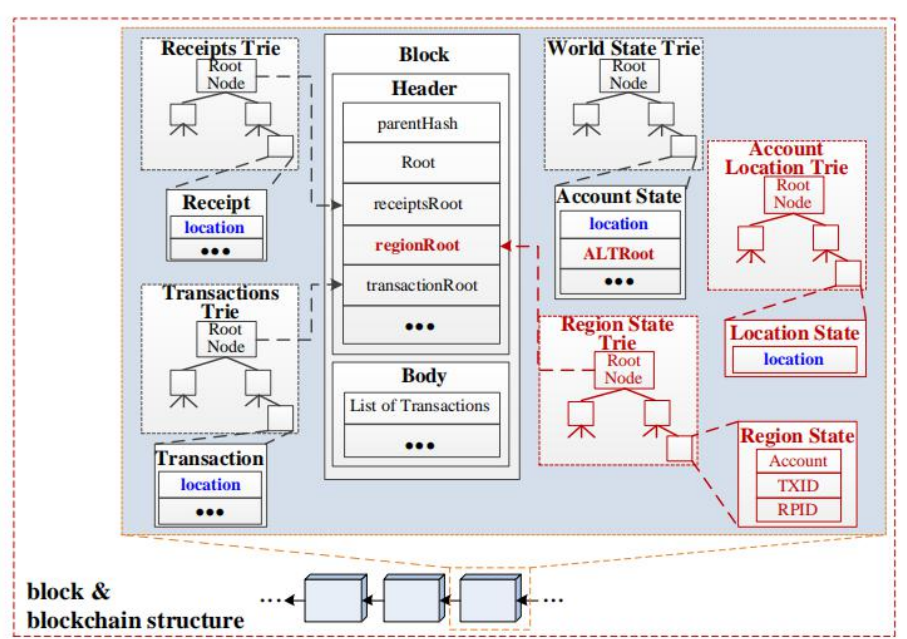
\includegraphics[width=\textwidth]{figures/树状区块链内部结构属性示意图.png}
	\caption{树状区块链内部结构属性示意图}
	\label{fig:树状区块链内部结构属性示意图}
\end{figure}

在现有的工作中,树状区块链在区域查询时可以对各种节点的各种属性进行高速索引,做到既有传统区块链所具有的安全性优势,同时也可以提高区块链的工作效率。但是,目前的工作仍有改善的空间,当前工作针对区域中的搜索可以高效完成,但当节点的地理位置发生较大移动时,此时必须要考虑将节点进行跨链移动,维持多链间的信息同步。简而言之,为使得树状区块链适配更广的适用范围,同时保持工作效率,需要基于现有的出租车调度系统,在其上实现树状区块链的跨链操作。

\subsection{智能合约}

区块链智能合约最早可以追溯到1994年,由Nick Szabo提出 。但真正受到广泛关注和应用是在比特币出现后。智能合约是一种基于区块链技术的自动化数据处理工具,它可以在不受任何第三方干预的情况下实现交易流程。在以太坊中,智能合约还具备信息系统和区块链之间接口的作用 。

智能合约的主要特点包括:
\begin{itemize}
    \item 自动执行:智能合约根据设定的条件和规则自动执行,并在执行完成后更新链上状态。
    \item 去中心化管理:智能合约不需要中心化机构来控制,而是通过代码规则和全网节点来实现管理。
    \item 不可篡改:智能合约一旦被写入区块链,就不能被篡改或删除。
    \item 信任机制:智能合约建立在去中心化的信任机制上,通过全网节点验证执行结果的真实性和正确性 。
\end{itemize}

智能合约的应用如今日益广泛,其可用于处理复杂的金融合约、物流、医疗和电子商务等领域,提高交易效率、降低成本和减少纠纷。 

\section{本文研究内容及贡献}

本文的内容结构如下:文章分为六章:

第一章首先介绍了基于树状区块链的出租车调度系统的应用背景与意义,之后介绍了相关技术的调研情况,最后总结了本文的研究内容及贡献。

第二章则主要针对树状区块链的部分功能实现做了说明,在源码仓库中增添了相应的注释说明。

第三章介绍了基于实验室以往工作而做的区域索引的树状区块链应用于出租车调度系统的复现实验的实验过程。

第四章介绍了对树状区块链应用于出租车调度系统的性能测试实验,验证多子链并行运行的性能负载情况。

第五章介绍了树状区块链的跨链资产转移功能。设计实验验证了树状区块链的跨子链资产转移功能的正确性,并测试了其性能。

第六章,在以上工作的基础之上,本文尝试对现有的出租车调度系统进行跨链交易的改进。现有的出租车调度系统仅支持一个子链内部的交易,针对乘客与车辆分处不同区域的实际应用场景,本文尝试对现有的出租车调度系统进行改进使其支持跨链的交易操作,并最终给出了一个简易的能够实现跨链交易的调度过程,设计实验验证了实现的正确性。



% !TeX root = ../thuthesis-example.tex

\chapter{go-ethereum的部分源码解读}

\section{整体结构}

go-ethereum的代码结构非常清晰,整个代码库主要分为以下几个部分:

\begin{itemize}
    \item accounts:这是管理以太坊账户的代码,包括账户管理、加密和解密、签名和验证等。
    \item cmd: 包含所有go-ethereum的命令行工具,如geth、abigen、bootnode等。
    \item core: 核心代码,包括区块链数据结构、区块链的实现、账户管理、交易执行等。
    \item crypto: 加密相关的代码,如私钥生成、签名等。
    \item consensus:这是区块链共识算法的实现,包括PoW(Proof of Work)、PoA、Ethash等。
    \item eth:以太坊网络协议的实现,包括区块同步、交易广播、状态传播和客户端协议等。
    \item internal:包含整个项目中使用的内部包。
    \item miner: 包含了以太坊矿工相关的代码,如挖矿、打包交易、广播区块等。
    \item node: 包含了以太坊节点相关的代码,如节点的启动、关闭、管理等。
    \item p2p: 网络层的实现,用于节点之间的通信。
    \item params: 包含了以太坊的参数配置,如区块链难度、网络ID、区块奖励等。
    \item storage:包含了以太坊的存储实现,如LevelDB等。
    \item rpc: 实现了以太坊的JSON-RPC API、WebSocket和IPC等。
    \item whisper: 实现了以太坊的whisper协议,用于点对点的消息传递,实现安全、私密的通信。
    \item trie: 包含了以太坊中使用的Merkle Patricia Trie数据结构相关的代码,如节点的添加、删除、查找等。
\end{itemize}

\section{部分核心源码的功能介绍}

由于我的实验目标与跨链与转账有关,故重点研究了树状区块链的结构,以及转账操作中涉及的代码内容。具体的代码注释已存入了我的毕设仓库当中。

图\ref{fig:树状区块链内部结构属性示意图}是树状区块链的内部结构属性示意图,展示了树状区块链的存储的各种属性,结合此图着重研究了区块链的区域索引的实现,树状多链结构的实现,区块汇总的实现以及跨链资产转移功能的实现。

\begin{figure}
	\centering
	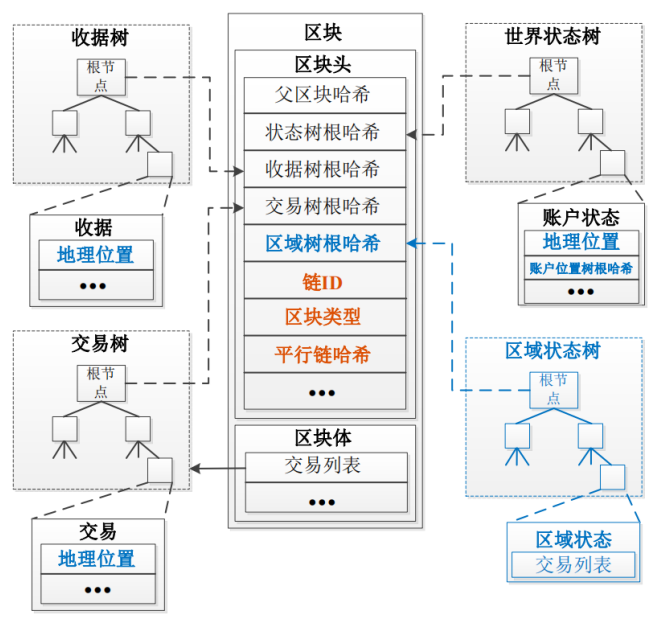
\includegraphics[width=0.6\textwidth]{figures/树状区块链结构属性示意图.png}
	\caption{树状区块链内部结构属性示意图}
	\label{fig:树状区块链内部结构属性示意图}
\end{figure}

\subsection{针对区域索引的说明}

首先是对创世块增加position的地理位置属性,创世块写入数据库并存储,实现存储创世块中的账户位置。

其次,对于account账户添加position的地理位置属性,同时实现获取账户位置的函数接口GetPosition,根据账户位置的hash值添加账户位置树;对于transaction交易添加position的地理位置属性。

实现并添加区域状态树,添加区域状态数据库,缓存区域状态,在miner中添加区域状态信息。区域状态树用于记录地理区块内的数据,便于地理信息的查询与相关数据的校验。

\subsection{针对树状多链的说明}

\begin{figure}
	\centering
	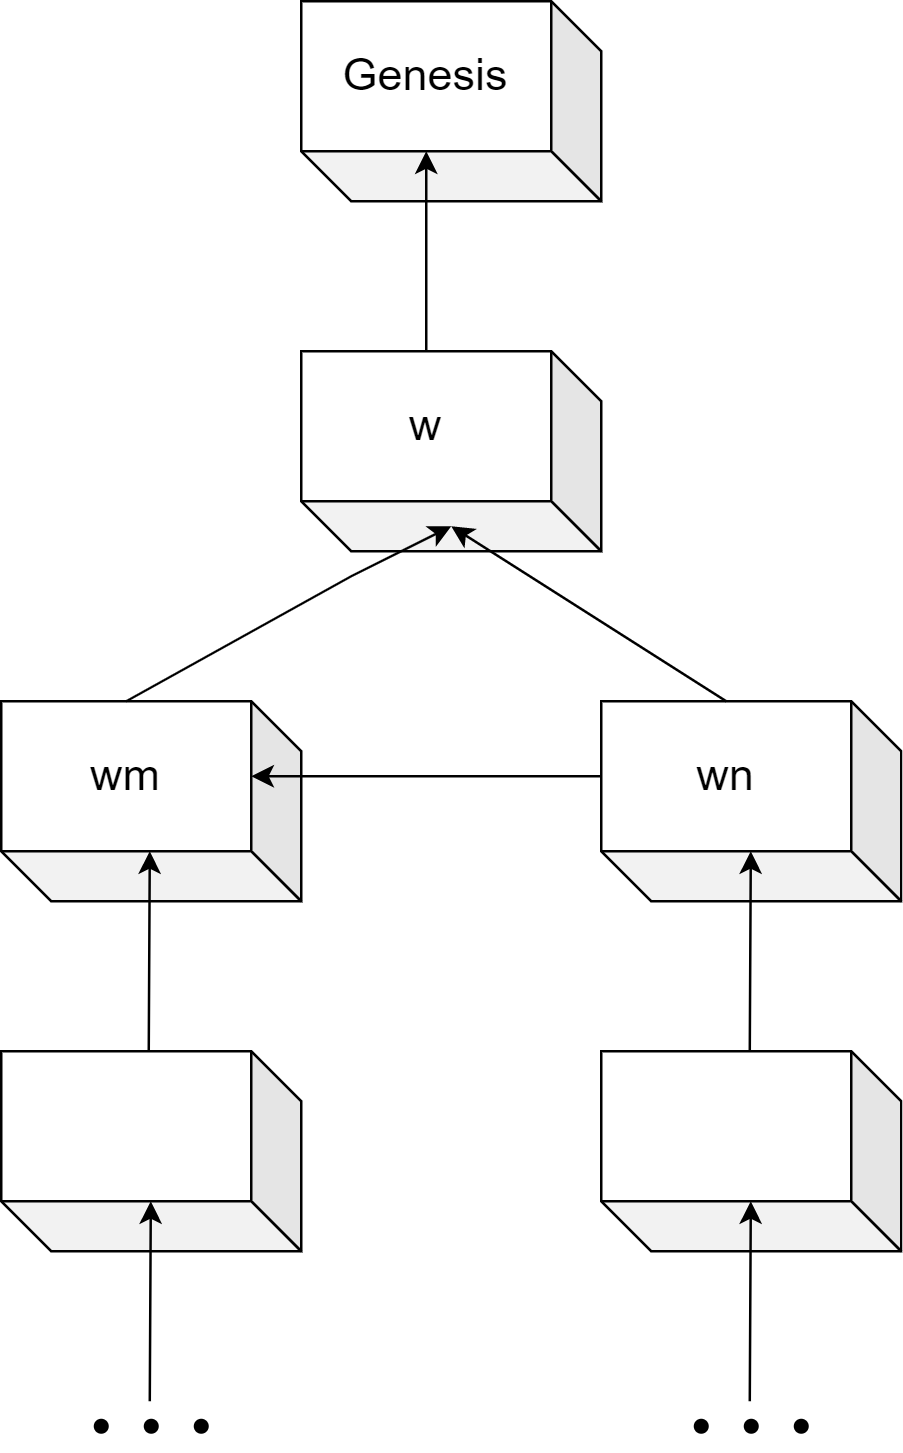
\includegraphics[width=0.4\textwidth]{figures/多链结构.png}
	\caption{树状结构}
	\label{fig:树状结构}
\end{figure}

将原本的单链结构变为多链结构,落实到代码中,添加了区块链内的链ID(chainID),区块类型(blockType)和平行链哈希(parallel Hash)。如图\ref{fig:树状区块链内部结构属性示意图}和图\ref{fig:树状结构}所示,链 ID(chainID)的作用是区分来自不同区块链的区块。区块类型是指支持区域索引的树状区块链将区块分为了三种区块:创世块、分支区块、普通区块。该属性即是指对当前区块类型的划分。平行链哈希则是分支区块不仅仅需要用父链指针指向自己的上层区块,同时还需要用一个平行链指针指向跟自己拥有相同父区块且Geohash编码的前n-1位相同的已产生的同层级分支区块。

\subsection{针对区块汇总的说明}

\begin{figure}
	\centering
	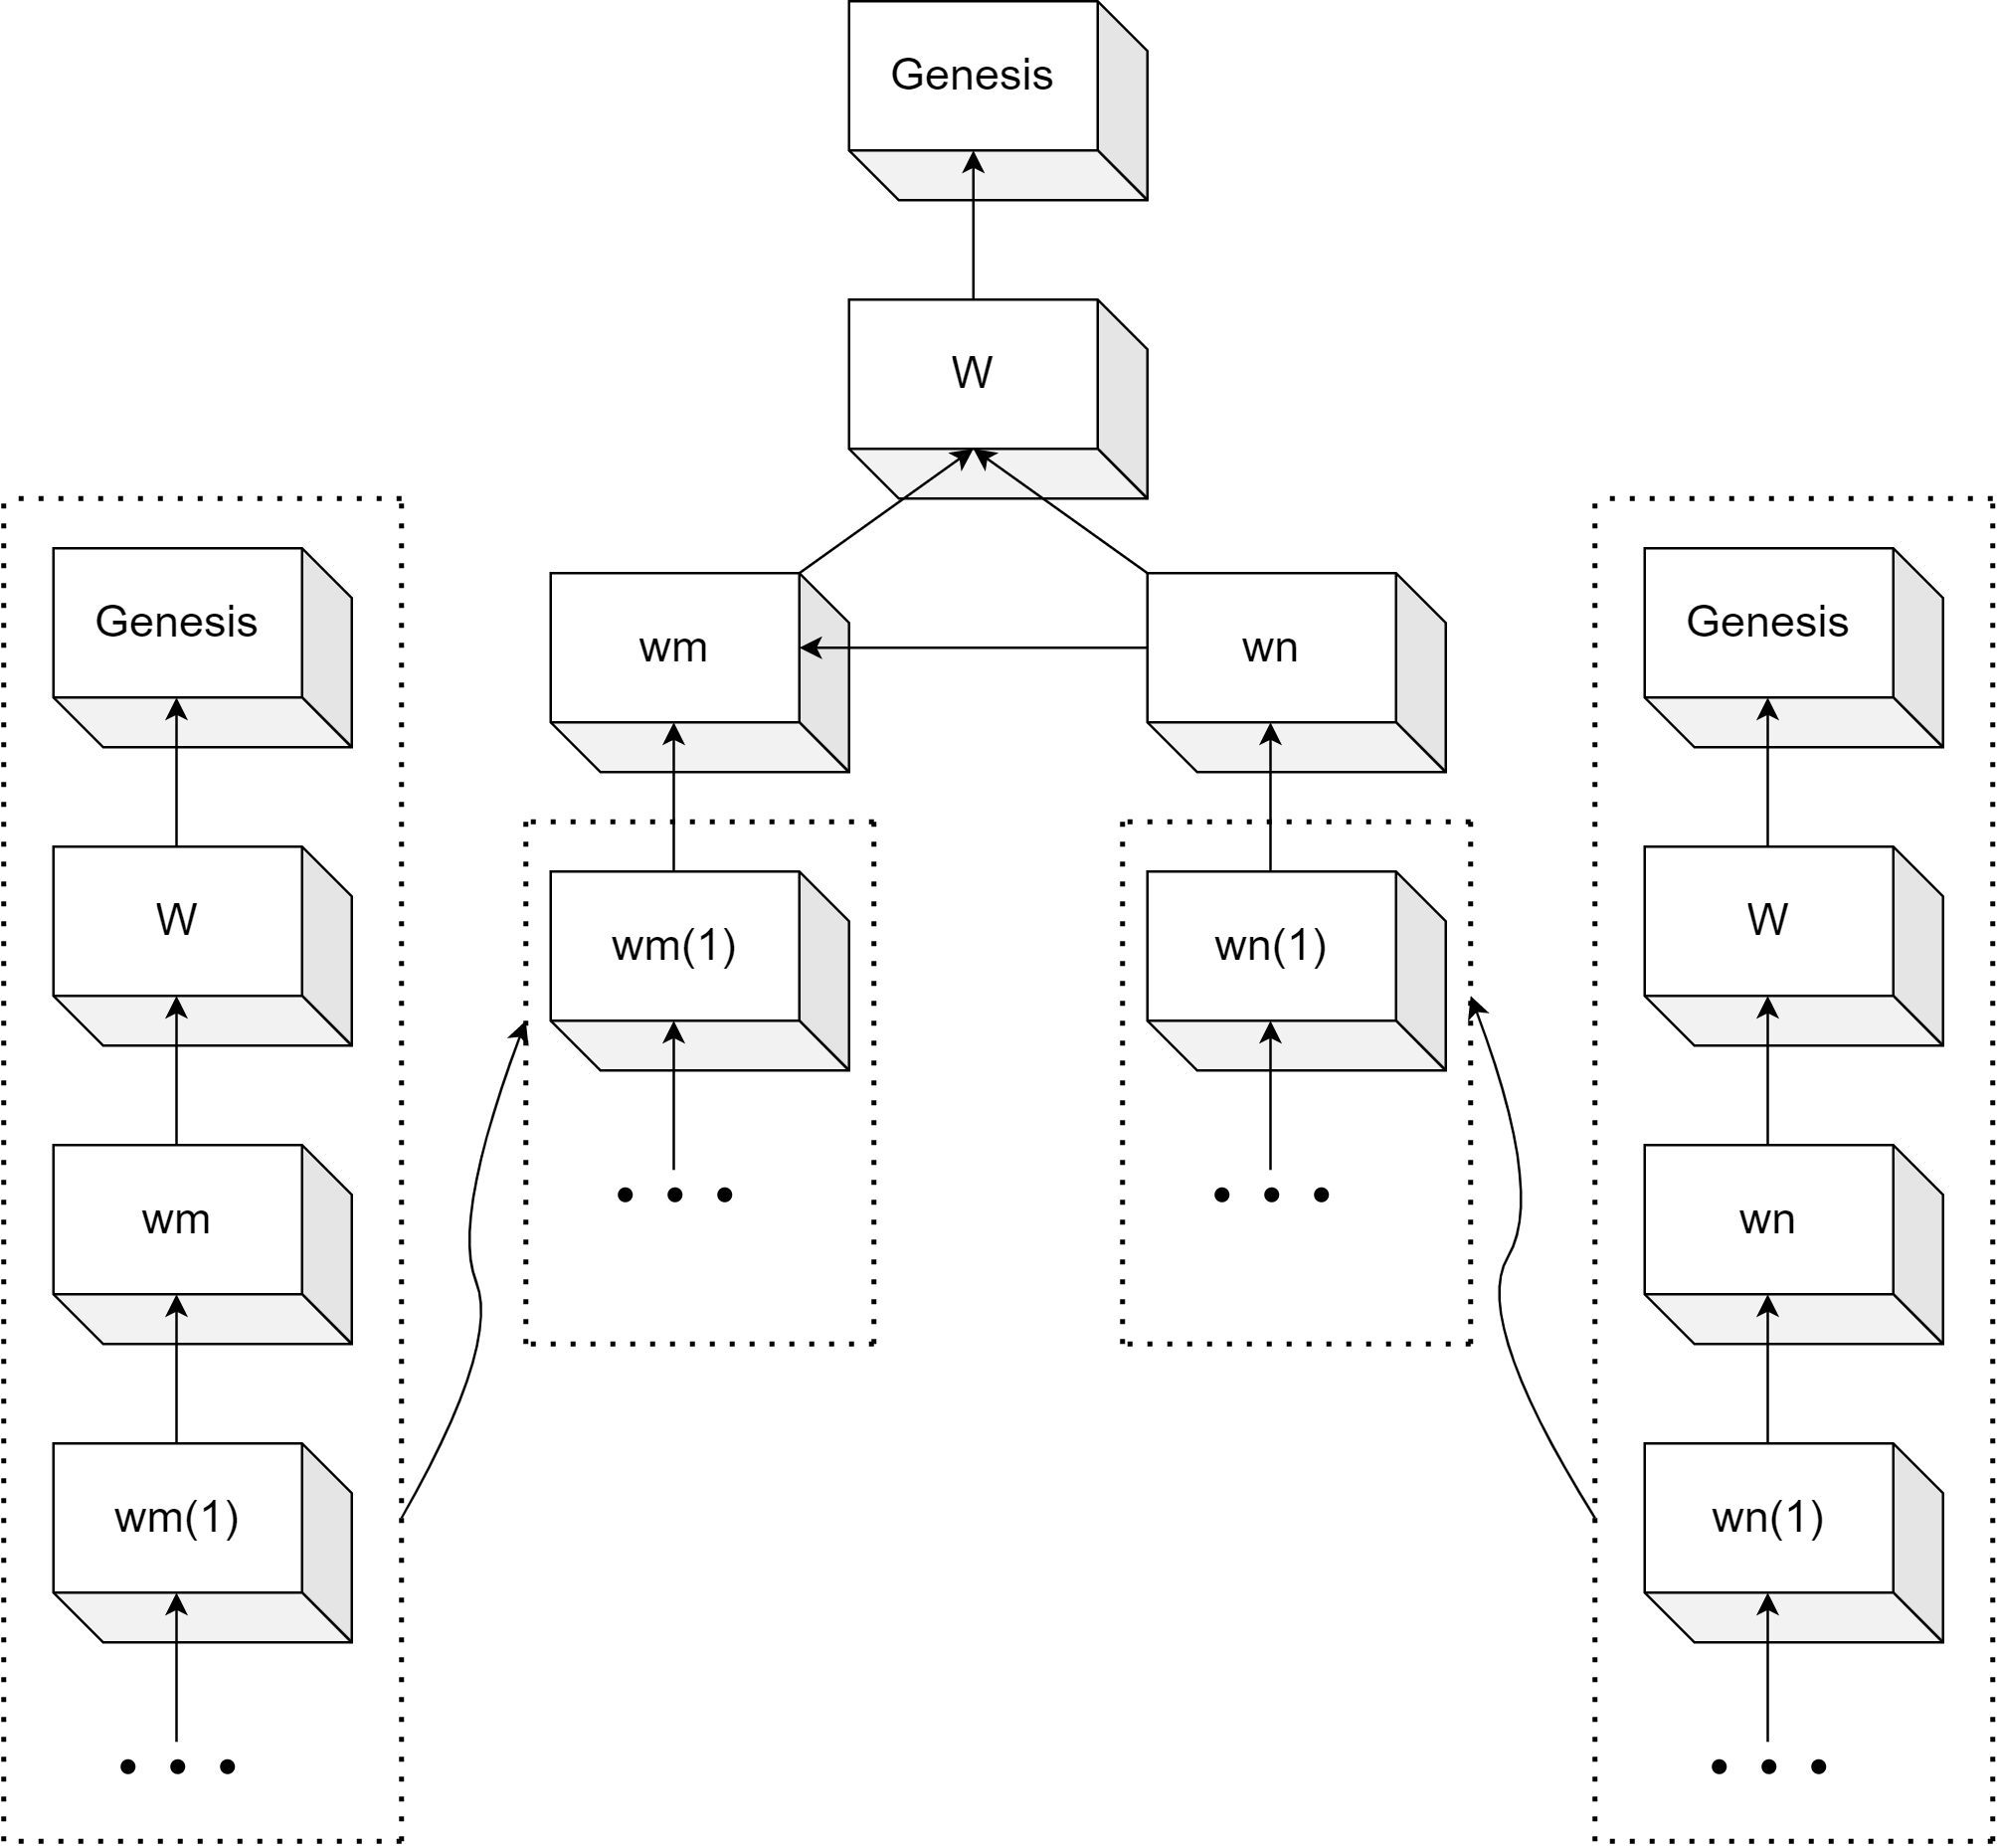
\includegraphics[width=0.8\textwidth]{figures/区块汇总过程示意图.png}
	\caption{区块汇总过程示意图}
	\label{fig:区块汇总过程示意图}
\end{figure}

节点中记录分支区块,并增加同步分支区块,区块汇总的方式,分支节点可以生成分支区块,分支区块写入区块链后,会根据regionid同步区块。

图\ref{fig:区块汇总过程示意图}为区块汇总过程示意图。分支节点在进行区块汇总时,按照子链地理区域独立汇总,最终可以将各子链中需要同步的区块都同步到分支区块中的对应的区域的分支上,此外,同步后的区块的内容以及其排列顺序都与待汇总子链相同,保证了各子链中交易顺序的不变性。

\subsection{针对资产转移的说明}

\begin{figure}
	\centering
	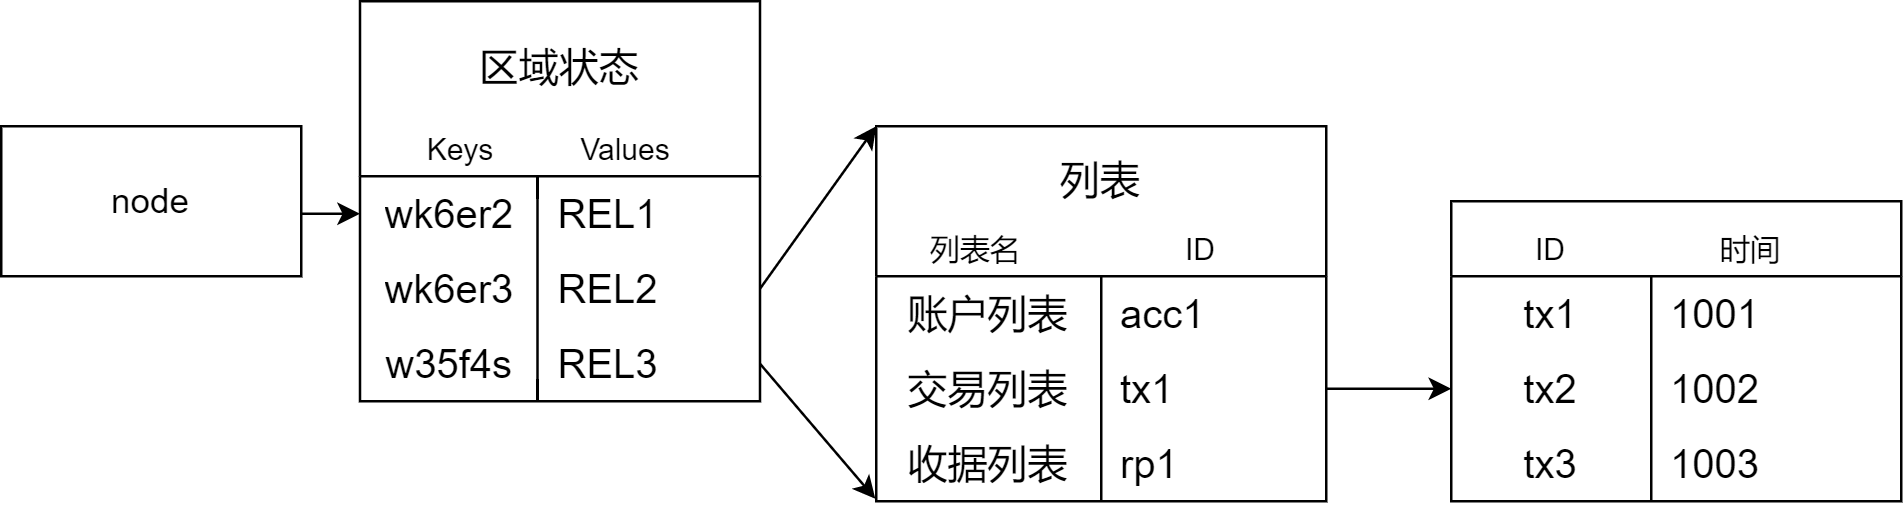
\includegraphics[width=\textwidth]{figures/交易列表.png}
	\caption{节点中资产转移列表相关结构}
	\label{fig:节点中资产转移列表相关结构}
\end{figure}

如图\ref{fig:节点中资产转移列表相关结构}所示,在分支节点中管理着资产转移交易列表,该列表结构中存储着子链发起的资产转移交易内容,此外对于添加进该列表的交易,代码还实现了交易的原子性操作。

资产转移交易被定义为特殊的交易类型,其设定为不需要消耗gas,此外,相较于传统交易,资产转移交易额外增加了一个自定义的txtype属性,列表中记录了该txtype属性以及对应的时间戳。

分支节点在同步区块时,若接受到含有txtype属性的交易,则判断此交易是否是资产转移交易,根据接收到的txtype值的不同进行后续的不同事件处理,包括目标链发起请求,来源链转出请求,目标链转入资金,来源链记录交易。

\section{本章小结}

本章对现有系统使用的树状区块链源码中的部分功能所涉及到的源码作了注释,详细说明在仓库中。

主要作用是方便后续工作者更好地理清代码逻辑,可以对整个系统的运作流程更为清晰。同时,也便于未来可能的对现有的底层源码的改进工作的进行。

% !TeX root = ../thuthesis-example.tex

\chapter{基于区域索引区块链的出租车调度系统复现}
本章的主要内容是实现基于区域索引的树状区块链的出租车调度系统的复现工作;在目前该课题已实现的出租车调度系统中,利用geohash编码存储地图数据,实现并部署了有路径规划以及车辆匹配的算法合约,并且使用Vue 2.JS作为前端可以表现出乘客与车辆的操作界面。其中用户可以通过实时地图信息获得自己的位置以及附近在线的乘客、司机等信息。乘客在发出乘车请求后,系统自动匹配附近的符合要求的车辆信息,司机在接到订单信息后,可以选择是否接受订单。司机接受订单后,进行路径规划。当车辆接到乘客时,乘客可以选择上车,而司机则是确认到达乘客上车地点。在抵达乘客目标后,乘客需要支付订单,确认订单支付后,调度系统完成。

复现工作大致分为两步:第一步是实现区域索引区块链的出租车调度系统的复现工作,该复现工作主要基于万琦玲的复现手册进行。第二步则是进一步实现基于树状区块链的区域索引出租车调度系统。

实验复现的过程已形成操作文档放入了我的毕设仓库当中供后来者参考。
 
本章节内容为大致介绍一下复现的流程,此外还有我在这一复现过程中所遇到的问题与解决方案,以及我对复现文档做出的改进与调整。当下的复现文档相较于初版大大提高了可理解性与可扩展性。

\section{区域索引区块链的出租车调度系统}

\subsection{环境配置}

操作系统 Ubuntu 22.04.1 LTS

虚拟机 VMWare Workstation Pro 17
	
一些JavaScript库:npm、truffle、node.js、ethereum、web3.js等 

区域索引区块链的二进制可执行文件(代码仓库中的 geth1 二进制可执
行文件)存放到/usr/local/bin 文件夹下

\subsection{实验步骤}

实验复现的过程,我已形成操作文档放入毕设仓库当中:

具体可以参考从《1 传统区块链初始化和启动》到《7 调度系统复现实验》的这一过程,其中本节重点说一下《7 调度系统复现实验》的过程,其余实验均为调度系统复现工作的前置测试实验,用于理解并测试系统的相关功能所用。

\subsubsection{初始化并启动区域索引区块链}

首先配置genesis.json,配置创世块文件,之后,命令行运行如下指令实现初始化区块链并启动区块链:

\begin{verbatim}
// 初始化区块链
geth1 --identity "MyEth" --rpc --rpcaddr 127.0.0.1  
--rpcport "8545" --rpccorsdomain "*" --datadir gethdata 
--port "30303" --nodiscover --rpcapi "eth,net,personal,
web3"--networkid 91036 init genesis.json
// 启动区块链
geth1 --datadir ./gethdata --networkid 91036 --port 
30303 --rpc --rpcaddr 127.0.0.1 --rpcport 8545 --rpcapi 
'personal,net,eth,web3,admin' --rpccorsdomain='*' --ws 
--wsaddr='localhost' --wsport 8546 --wsorigins='*' 
--wsapi 'personal,net,eth,web3,admin' --nodiscover 
--allow-insecure-unlock --dev.period 1 --syncmode='full'
console
\end{verbatim}

指令参数解读:


\begin{itemize}
    \item identity "MyEth":	设置节点的标识。
    \item rpc:					启用RPC服务器。
    \item rpcaddr 127.0.0.1:	指定RPC服务器的IP地址。
    \item rpcport “8545”:		指定RPC服务器的端口号。(外部程序可以使用该端口接入区块链,进而借助 JSON-RPC API 或者 web3.js 库和区块链进行交互。)
    \item datadir gethdata:	指定链上数据存储目录。
    \item port “30303”:		指定节点端口号。
    \item rpcapi “eth,net,personal,web3”:启用RPC API。
    \item networkid 91036:		指定网络ID。
    \item ws:		启用WebSocket服务器。
    \item wsaddr 'localhost':  将WebSocket服务器地址设置为localhost。
    \item wsport “8546”:		将WebSocket服务器端口设置为8546。
    \item init genesis.json:	使用genesis.json文件初始化区块链。
\end{itemize}


启动区块链后,终端中将出现 JavaScript 控制台。此时,区块链已经启动完毕,可以在控制台创建账户并进行测试;需要注意的操作有:1. 创建账号后,需要将账户信息添加到genesis.json的alloc字段中,同时赋予创建的账号初始余额,以方便后续的调度实验的进行;2. 每次启动区块链都要解锁账户,否则账户无法部署合约,进而系统无法工作

在打开的控制台中输入exit退出控制台,然后删除目录./gethdata/geth。随后,再运行一次初始化区块链和启动区块链的代码,此操作是为了强制重新加载创世块文件。此时,所有账户应该都有余额了。可以用eth.geBalance(账户地址)来检查余额,余额显示正常则表明区块链已成功建立。

\subsubsection{部署合约}

这一步,我并未遇到什么问题,主要介绍一下系统所用到的两个合约:

\begin{itemize}
    \item StoreMap.sol:主要有存储各种地图数据的数据结构以及查询方法,此外还提供了A-Star寻路等算法的实现
    \item StoreTraffic.sol:主要提供了司机和乘客的各项信息的管理,导航结果,以及基于geohash的对于调度车辆的查询算法
\end{itemize}

在部署合约的这一步操作中,源复现文档仅给出了合约编译后的abi以及bytecode内容,我在文档中添加了Remix Desktop编译合约并记录编译结果中的ABI字段进行压缩转义,同时记录bytecode字段的这一过程。

将二者复制到部署合约的代码模板中,并将两份编辑好的模板复制到正在运行geth1的 JavaScript命令行后,合约部署的请求就已经提交至交易池。开始挖矿并密切观察控制台输出,直至获取合约地址后,说明合约部署成功。

\subsubsection{上传地图}

这一步是直接调用了现有系统的上传地图的JavaScript 脚本文件,注意需要修改StoreMap的合约地址,初始的执行数据提交的账号的公钥地址,以及要上传的地图数据文件(可选,在后续实验中修改了地图数据文件)运行该脚本,直至终端输出“地图数据上传完成”字样后,结束挖矿。此时,地图数据便已成功的上传到了区块链上。

\subsubsection{更改文件以加入账户信息}

仓库文件夹\verb|investigation-cjzhuang2020/cjz_underg_2021_09|

按照文档说明,在上述路径中找到:乘客账户文件,车辆账户文件,StoreMap合约地址文件StoreTraffic合约地址文件,乘客的位置信息文件(包括乘客的账户信息,初始位置,调度起点,调度终点),以及车辆的位置信息文件(包括车辆的账户信息,车辆的初始位置)。

将上述文件进行修改后,即可启动测试。

\subsubsection{启动实验}

启动挖矿,新建两个终端,准备启动车辆客户端和乘客端的测试脚本。

\verb|python3 vehicle_test.py|

\verb|python3 passenger_test.py|

看到如图\ref{fig:车辆端初始界面}中的提示,说明车辆位置上传成功:

\begin{figure}
	\centering
	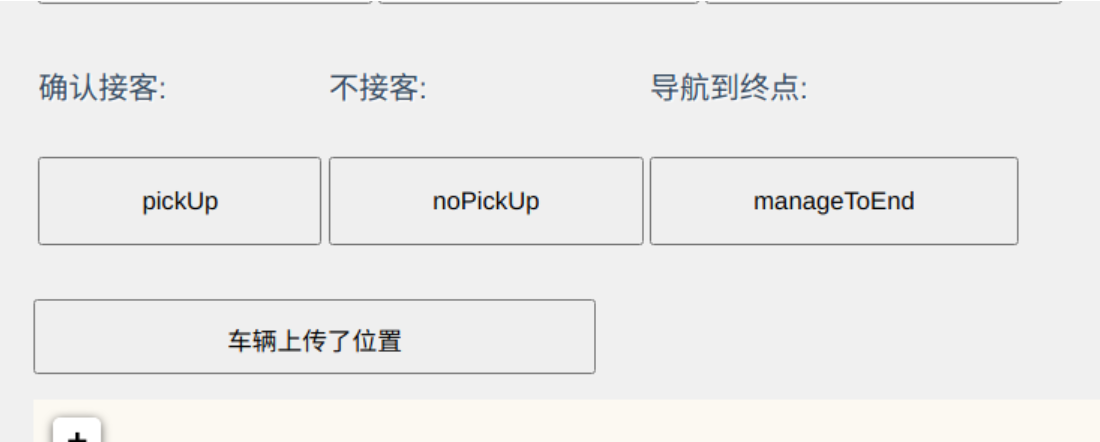
\includegraphics[width=0.9\textwidth]{figures/车辆端初始界面.png}
	\caption{车辆端初始界面}
	\label{fig:车辆端初始界面}
\end{figure}

被selenium控制的浏览器会进行一系列的操作,当司机端询问:Whether to pick up the passenger时,点下图\ref{fig:车辆端界面}中的pickUp按钮接起乘客,即可完成后续的调度步骤:

\begin{figure}
	\centering
	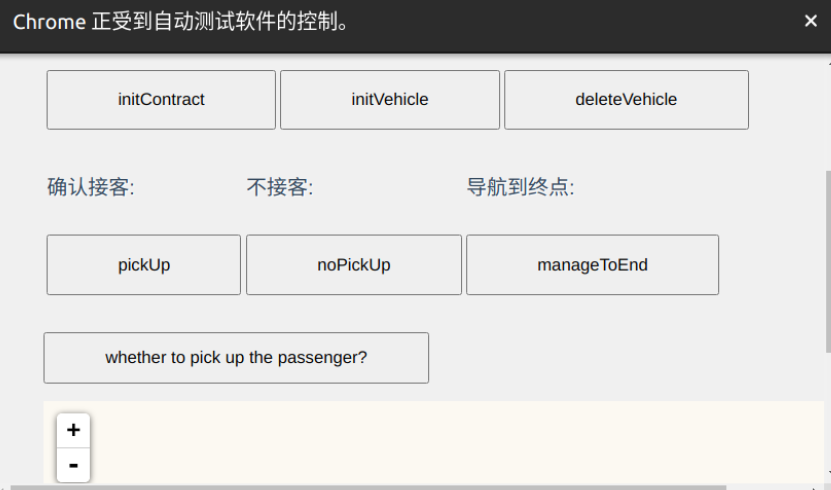
\includegraphics[width=0.9\textwidth]{figures/车辆端界面.png}
	\caption{车辆端界面}
	\label{fig:车辆端界面}
\end{figure}

最终,乘客被送达目的地,并在支付订单之后乘客端的测试程序结束运行:

\begin{figure}
	\centering
	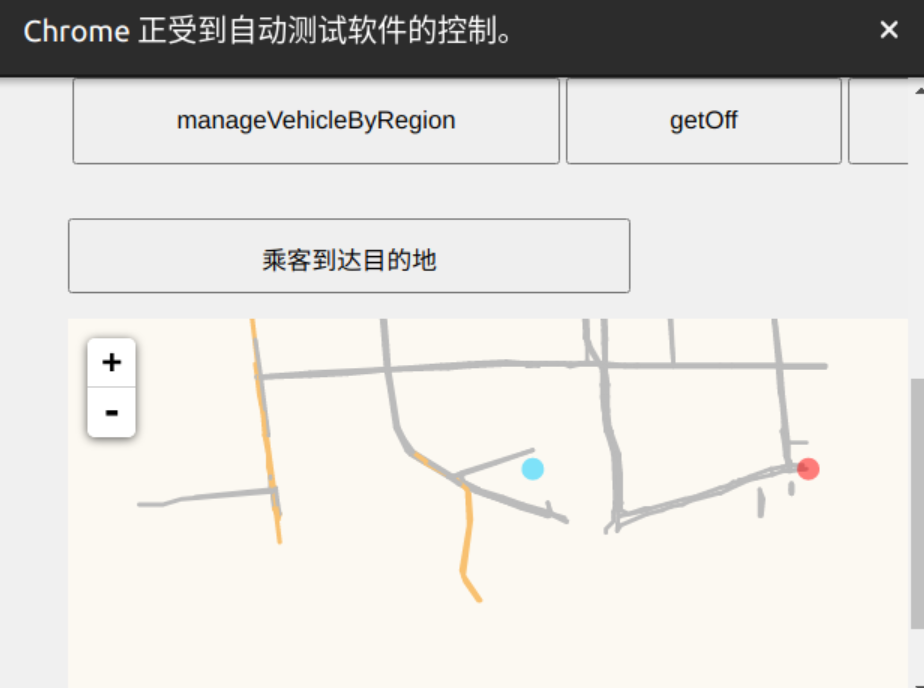
\includegraphics[width=0.9\textwidth]{figures/乘客端界面.png}
	\caption{乘客端界面}
	\label{fig:乘客端界面}
\end{figure}

\section{区域索引的树状区块链的出租车调度系统}

上面的实验是在一条链上进行的复现实验,主要基于geth1进行,而本实验是实现区域索引的树状区块链的复现实验基于geth-tree完成。
	
大体操作基本同上,详情参见仓库里的《10 部署在geth-tree上的出租车调度系统复现实验》文档,这里主要介绍一下不同于上面实验的操作。

启动过程和原来的一致,只是启动文件根据区块链的不同有所变化,主要是regionid和position的变化。对于不同的账户而言,所处不同的子链,其对应的regionid和position也应不同,此外,为了支持对应的实验进行,还上传了全新的地图数据文件。

\section{问题及解决方案}

原版的复现手册中有着许多未说明清楚的部分,此外,操作步骤也并不完整。本小节主要介绍我在复现过程中遇到的问题以及解决方案。

\subsection{节点连接的问题}

在进行多节点连接时,发现无法同时运转两个节点,经过多次尝试,最终发现两个节点之间net.peerCount为0,这表明二者之间并未连接。

解决方案:复现手册中所说的需要把Node1中的Key文件复制到Node2中。实际并不明确,事实上,将gethdata/keystore文件夹下的内容复制过去,则表明二者之间有着相同的账户信息,因此,初始的创世块中也应初始化相同的账户余额。我将两个文件夹中的genesis.json信息同步后,将Node1文件夹下的keystore文件夹复制到Node2中。此时节点相互连通,问题解决。

\subsection{合约有关问题}

原版复现手册中仅仅给出了部署合约的模版代码,并未对其进行说明,此外也未对合约编译后的abi以及bytecode内容进行说明。我用Remix Desktop编译了合约,并记录了编译结果中的ABI字段进行压缩转义,同时记录了bytecode字段。

\subsubsection{编译合约}

我使用Remix Desktop和truffle两种方式实现了智能合约的编译。

首先是Remix Desktop,编译完成后,切换到编译选项界面,点击“Compilation Details”按钮,即可观察编译结果的详细信息,获得编译结果后,需要提取其中的应用程序二进制接口(ABI)和以太坊虚拟机字节码(bytecode)信息,需要妥善记录保存。然后是truffle,需要配置对应版本的truffle,然后在命令行中运行编译truffle compile即可得到编译结果。

\subsubsection{合约的应用}

在终端中实现智能合约的调用,需要特别关注对应的区块链网络端口以及需要获取对应的contractAbi文件,在修改完合约之后要及时更新对应的contractAbi文件,否则合约会调用失败。

此外,在部署合约时,还需要注意在将合约上转至对应的区块链上时,send的信息需要position满足位于当前的子链管辖范围之内,矿工在处理交易信息时,会提取出其中所包含的position信息,若判断不满足当前位置范围,则拒绝交易。

调用合约的示例如下:

\begin{verbatim}
const fs = require('fs');
const Web3 = require('web3');
let web3 = new Web3(new Web3.providers.WebsocketProvider(
"ws://127.0.0.1:" + PORT));

//Map contract
let mapContractAddress = '0x...';
let mapContractAbi = JSON.parse(fs.readFileSync(
'./mapContractAbi.json', 'utf-8'));
let mapContract = new web3.eth.Contract(
mapContractAbi, mapContractAddress);

//Traffic contract
let trafficContractAddress = '0x...';
let trafficContractAbi = JSON.parse(fs.readFileSync(
'./trafficContractAbi.json', 'utf-8'));
let trafficContract = new web3.eth.Contract(
trafficContractAbi, trafficContractAddress);

trafficContract.methods.example().then((res) 
=> {/* 
any code
*/});
\end{verbatim}

\subsubsection{合约的错误总结}

在我的复现过程中,遇到了许多合约上相关的问题,且每次问题的定位都给我带来了较大的麻烦,因此,这里整理了一下常见的可能会遇到的合约问题,便于后续工作者查验:

\begin{enumerate}
    \item 合约的编译问题。出现合约问题要首先检查合约是否正确编译,且调用的Abi和bytecode是否正确;此外,还要重点注意对应的ContractAbi文件是否更新,这是容易被遗忘的操作。
    \item 需要注意合约部署时是否正确部署。例如,合约部署时,管理员账户是否正确,position是否满足子链范围,gas是否足够等问题。
    \item 合约调用中的问题。需要注意合约地址是否正确,若要定位出现问题的合约函数,则可以通过合约函数的function(error)调用来实现定位。
    \item 在进行合约交互时,需要注意区块链启动时,是否允许WebSocket协议连接(区块链启动时的--ws操作),启用了WebSocket协议连接后,才可以进行上述实例代码中的操作。
\end{enumerate}

\section{本章小结}

本章介绍了使用区域索引区块链以及区域索引树状区块链来进行出租车调度系统实验的复现工作。大致介绍了复现的步骤,验证了复现工作的正确性,最后说明了复现过程中所遇到的问题与解决方案。
% !TeX root = ../thuthesis-example.tex

\chapter{基于树状区块链的出租车调度系统测试}

\section{实验说明}

前文中提到,现有的树状区块链添加了geohash编码的地理位置属性,提供了区域搜索的功能,本章实验就是测试现有的树状区块链在实际的出租车调度应用中的表现。

以第三章所描述的树状区块链的复现实验为基础,构建基于实际地理位置的多链区块链,并运行出租车调度系统,通过设定好乘客和车辆的初始账户数目后进行实验,统计乘客端和司机端在运行整个调度系统中所消耗的时间并将其可视化。测试树状多链区块链多链同时运行相较于单链运行的性能表现,分析对于机器的负载要求。

同时,我还对现有仓库中的测试脚本进行了修改与重构,并提供了详细的操作说明,简化了部分操作,提高了代码的复用性,也方便后续工作者的进一步的实验。

\section{实验设计介绍}

在本章实验中,树状区块链的构成为一条虚拟父链,对应的地理位置为真实世界地图中Geohash编码前缀为wx4e的区域,其下有4条子链,对应的地理位置分别为Geohash编码前缀为wx4en、wx4ep、wx4eq和wx4er的4个区域。我在每条链中均分配了多位司机和乘客账户,所有司机的初始位置均相同,所有乘客之间的出发地点和目的地也相同。以上地点的选点工作基于蒙思洁完成的真实地图信息提取与筛选工作进行,已提前确保选择的路线可以在真实世界地图上导航成功。

本章实验主要使用JavaScript脚本来模拟司乘交互的整个过程。具体流程如图\ref{fig:出租车调度系统的运行流程图}所示。总体来说,司机端模拟脚本负责将司机的公钥地址,初始位置上传到区块链上,之后,便是监听一系列与乘客交互的合约中定义的事件,最终按顺序完成接单,导航,确认完成订单这一系列行为。乘客端的模拟脚本负责将乘客的公钥地址,起点位置和目的位置上传到区块链上,之后每隔一段时间将有一名乘客提交乘车请求,并搜索周围车辆账户,选取离乘客出发点曼哈顿距离最近的车辆账户相应匹配,尝试建立连接;若车辆目前已被占用,则等待一段时间后,继续重复上述操作。在乘客与车辆建立连接后,便是调用一系列合约中的事件函数进行交互,最终按顺序完成上车,到达目的地付款,确认完成订单这一系列行为。

\begin{figure}
	\centering
	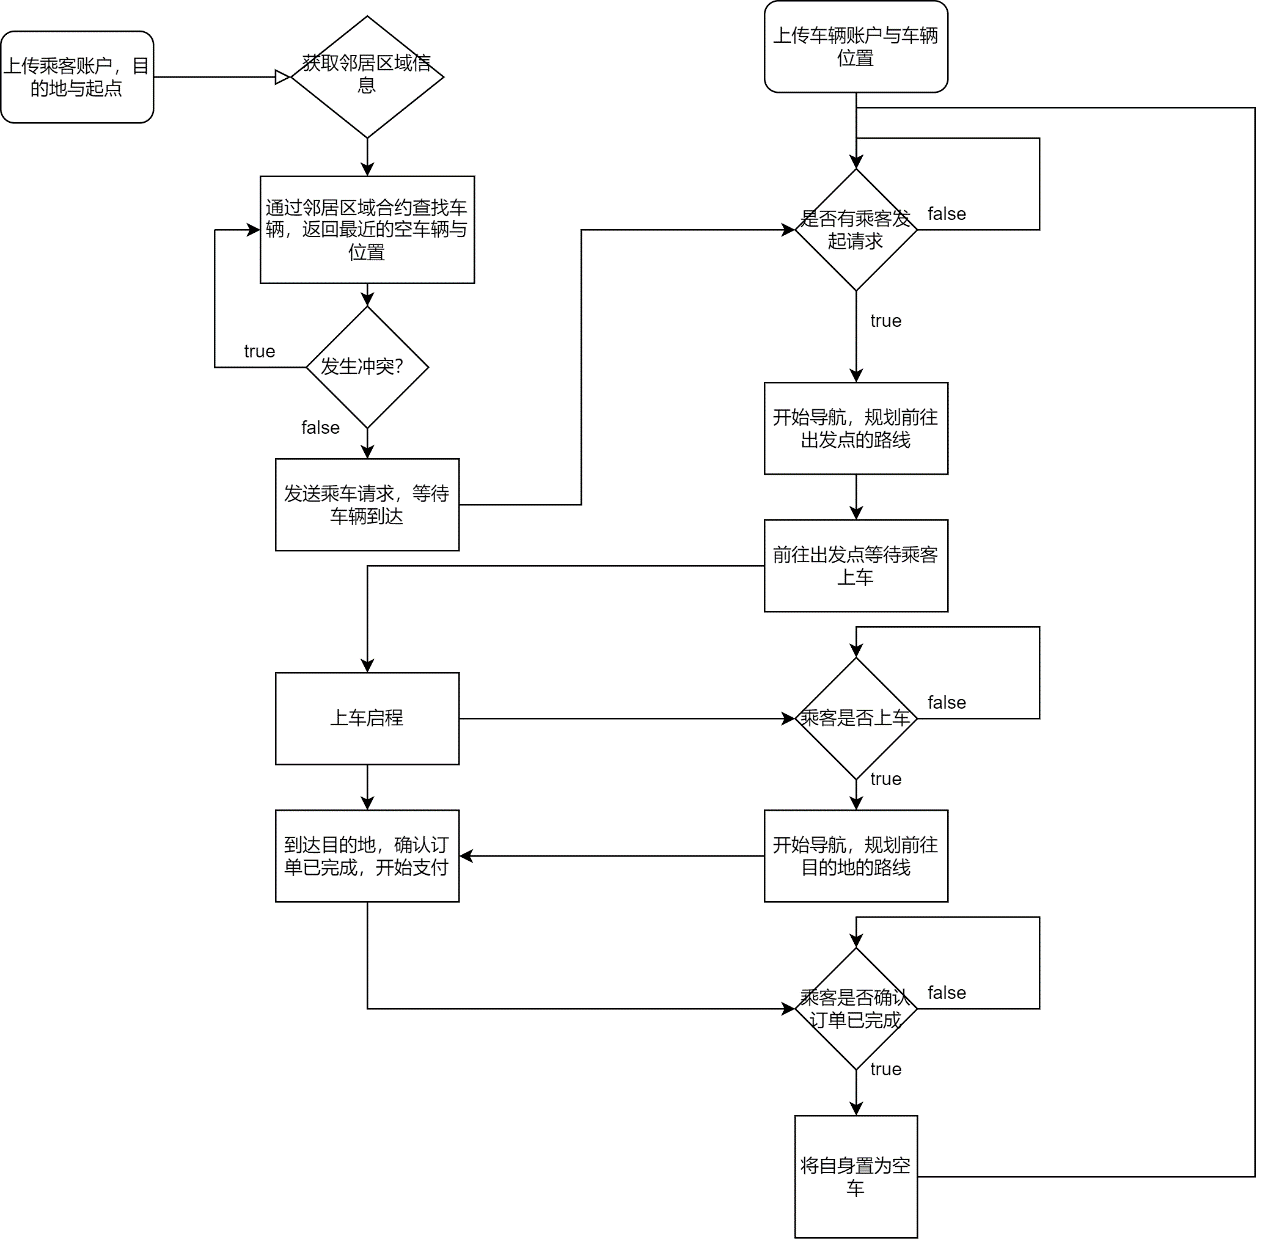
\includegraphics[width=\textwidth]{figures/出租车调度系统的运行流程图.png}
	\caption{出租车调度系统的运行流程图}
	\label{fig:出租车调度系统的运行流程图}
\end{figure}

\section{实验数据设计}

本实验的一个重点便是在于乘客与司机的初始位置的确立。实验中在4条链的区域内,各选择了一条能够进行双向导航的路径,并把该路径的起点作为乘客的起点,终点作为乘客的目的地,司机的初始位置则设为了乘客的目的地,即该路径的终点。这样在运行调度系统时,车辆先完成一次由路径终端到路径始端的导航,接到乘客后,车辆就再完成一次由路径始端到路径终端的导航。经多次实验测试,最终挑选了如表\ref{测试数据集地理位点}中的点位数据来进行本章实验。

\begin{table}
    \centering
    \caption{测试数据集地理位点}\label{测试数据集地理位点}
    \begin{tabular}{cccc} \toprule
        区域Geohash前缀 & 乘客起点        & 乘客终点        & 司机初始位置      \\    \midrule
        wx4en       & wx4enscgue5 & wx4enrq9mm9 & wx4enrq9mm9 \\
        wx4ep       & wx4epb8scg1 & wx4ep8e5gw0 & wx4ep8e5gw0 \\
        wx4eq       & wx4eq7rgmxk & wx4eqt6u0vu & wx4eqt6u0vu \\
        wx4er       & wx4erd4xkyz & wx4erw9rmze & wx4erw9rmze \\
        \bottomrule
    \end{tabular}
\end{table}

在链中初始化账户信息,并将其按照1:2的比例分为车辆账户与乘客账户,在本次实验中,参与测试的账号共有48个。其中车辆账户16个,每条链中分配4个,乘客账户32个,每条链中分配8个。划分方式,将eth.accounts中管理员外的账户,平均分配到了四条子链做当前链的活跃账户。

仓库中存有快捷分配账户的脚本,此外,分配到各链当中的信息也会以JSON格式存储到本地文件当中,便于后续查看账户具体信息和脚本读取所用。

\section{进行多子链的实验测试}

\subsection{编译并配置树状区块链}

下载实现的树状区块链的源码之后,配置好需要的编译环境,之后在源代码目录终端输入make geth,待编译完成后可以在build/bin目录中找到生成的geth可执行文件,在此实验中,将其重命名为了geth-tree后复制到了/usr/local/bin目录中,此后便可通过geth-tree指令来建立并启动区块链。

\subsection{进行实验}

本节实验的测试代码以及详细的操作文档均收录在本人的毕设仓库中,因此,本节主要介绍一下实验的大体过程。

\subsubsection{四子链并行实验}

\begin{enumerate}
    \item 准备测试用的司乘数据,运行脚本自动执行账户划分工作,结果存于仓库中的json格式的文件中
    \item 按照操作顺序启动四条子链,构建四子链网络,注意此步骤需要确保四个子链中./gethdata/keystore文件夹下均拥有相同的48个账号,并且账号均处于解锁状态(可以运行脚本自动操作)
    \item 在四子链上分别部署合约,并在乘客端和司机端的测试脚本中更新合约地址
    \item 上传地图文件
    \item 依次启动四条子链开始挖矿,同时运行乘客端和司机端的测试脚本,等待测试结束
    \item 对得到的输出文件进行可视化处理
\end{enumerate}

\subsubsection{四子链分别进行单独的单链实验}

对四条子链均分别进行单独的单链测试并取四条链结果的平均值。分别测试单链中含有12个账户(4个司机8个乘客)时,平均每个订单司机端所消耗的时间。

\section{结果分析}

本章测试统计了车辆端的时间戳,实验结束后,从输出的文档中获取上述的耗时数据,对其进行计算和可视化的处理,其可视化结果如图\ref{fig:车辆端每个账户单次调度的耗时}所示。图中,展示了四子链并行运行和分别单独运行四条子链的平均值的测试结果。

% \ref{fig:乘客端平均每个账户单次调度的耗时},
% \begin{figure}
% 	\centering
% 	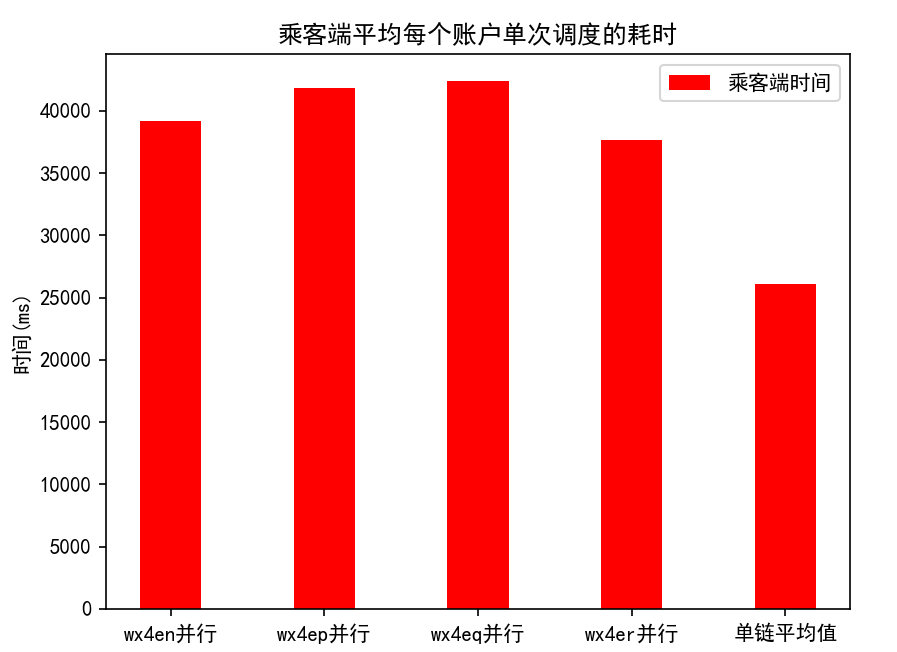
\includegraphics[width=0.8\textwidth]{figures/乘客端平均每个账户单次调度的耗时.png}
% 	\caption{乘客端平均每个账户单次调度的耗时}
% 	\label{fig:乘客端平均每个账户单次调度的耗时}
% \end{figure}

\begin{figure}
	\centering
	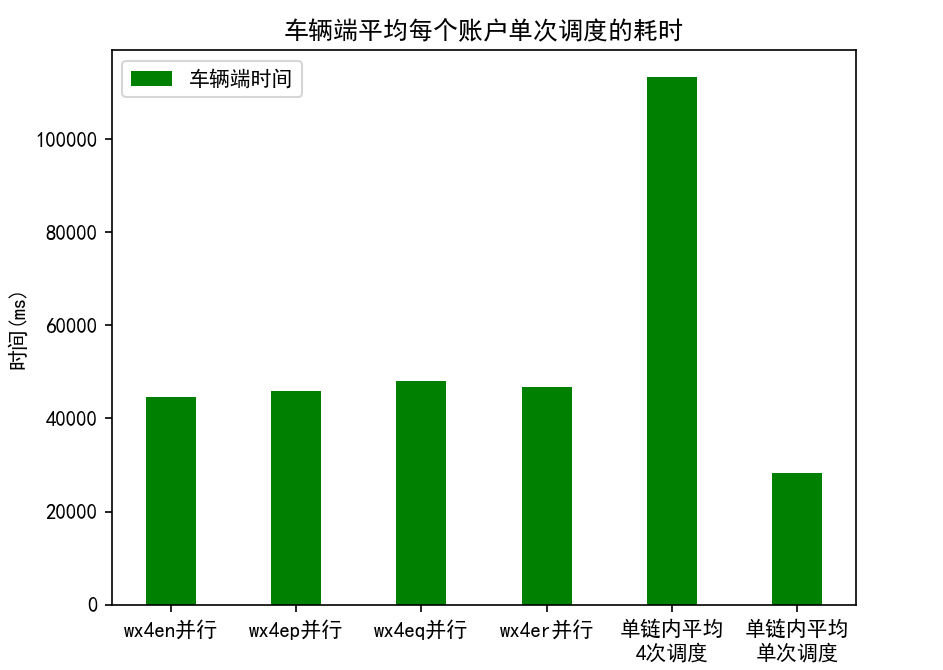
\includegraphics[width=0.9\textwidth]{figures/车辆端每个账户单次调度的耗时.png}
	\caption{车辆端每个账户单次调度的耗时}
	\label{fig:车辆端每个账户单次调度的耗时}
\end{figure}

分析图中结果可以看出,虽然并行运作时平均单次调度的耗时相较于单链时增多,但是若考虑是单个链中的48个账户(16个司机与32个乘客账户)的总耗时情况时,此时树状区块链的总耗时要远小于单链结构的情况,证实了树状区块链在车联网应用中有着良好的前景。

此外,从另一方面来看,四条子链可以并行运行出租车调度系统,但是其多链同时运行所产生的开销,也会制约树状区块链的综合性能,在后续的应用中,需要充分考虑机器的硬件配置、网络带宽、存储能力等方面,以确保系统的稳定性和安全性。

\section{本章小结}

本章主要介绍了树状多链区块链应用到出租车调度系统上的测试实验。首先,阐述了实验的设计思路;之后,以流程图的形式给出了实验的大致流程,并通过javascript脚本来模拟乘客端与车辆端的交互行为;然后是实验数据的确立,经测试选出了可以进行双向导航的测试节点,并在四条测试子链中部署了相同数目的车辆与乘客账户。接着,本章给出了实验的大致操作流程,并对结果进行了一定的分析讨论,证明了树状区块链的结构的优越,但同时也注意到为了确保系统的稳定高效,需要机器的硬件配置、网络带宽、存储能力等方面有较为优秀的配置。


% !TeX root = ../thuthesis-example.tex

\chapter{基于树状区块链的跨链资产转移测试}

\section{实验说明}

现有的树状区块链以区域搜索区块链为基础,旨在解决车联网中节点过多,传统单链结构在面对大量节点时开销过大的问题。其设计按照Geohash编码的地理区域划分的具备区域地理位置状态特性的树状多链结构,根据Geohash编码的前缀匹配,表示父链与子链,形成了一个树状多链的结构。

应用到车联网当中,大部分车辆节点是树状结构的叶节点,用于维护区块链结构的节点不能随意改变其所属区域。但是车辆具有移动性,其不仅仅只是在其所属的区域内部活动,还存在从一个区域进入到另一个子链所管辖的区域的这种实际情况。此时,车辆账户进入到了新的一条子链当中,但是这条新的子链目前并不具备车辆账户的各种信息记录,且车辆账户在新链中资产为0,此时发送交易,便会因为账户余额不足而失败。为了能满足车辆账户的这种可移动性,在树状区块链中,当一个账户位置发生了跨子链(跨区域)的这种移动时,账户需要向一个管理账号发送一种特殊的交易,管理账户在接收到该交易时,将转移账户的资产余额从原先的子链中,转移到目标子链中,以此来实现账户跨子链时的资产的一致性。之后,账户便可以正常进行如发送交易等与区块链的交互操作。在树状区块链中,同一个账户同时只允许在一条子链中有资产余额,此时该链便被称为该账户的活跃链。

需要注意的是,不同于传统区块链的跨链资产转移,传统区块链的跨链资产转移大部分是为了实现不同区块链上资产的交换,其本质是针对不同记账体系之间资产转移过程,此时,或者整个转移过程依赖于可信的第三方,如跨链桥、跨链协议,或者需要对区块链进行结构上的扩展,如实现侧链。本节提出的跨链资产转移也可以理解为是跨区域的资产转移,是整个树状结构中的子链之间的资产的相互转移。

本节要进行的实验测试,便是针对树状区块链的这一跨链转账功能的测试,主要测试目标为跨链转账功能的正确性及其性能表现。

\section{结合源码分析实验}

关于跨链资产转移的代码实现主要在eth/handler.go中的handleMsg函数中,在这个函数中,实现了检索并解码传播新的区块时需要进行的操作。若想进行跨链资产转移,只有当前区块是分支区块,在接收到了叶子区块的请求时才会进入跨链资产转移的判断。此时,该交易信息需要提交含有txtype属性值的一个变量,若其为1,则此时分支节点在验证后将新的交易添加到pending列表中,记录\verb|Tx_request|的请求;若其为2,则此时分支节点会根据发送方的地址和输出链将\verb|Tx_out|与相应的\verb|Tx_request|进行匹配。若其为3,则此时分支节点根据收到的接收方的账户地址和输入链,将\verb|Tx_in|与相应的\verb|Tx_request & Tx_out|相匹配。同时,为了维护整个过程的原子性,分支节点会验证从转账请求开始的全过程(验证上一步交易的hash信息)。

\section{资产转移过程的事件介绍}

\begin{enumerate}
    \item 跨区域资产转移请求交易事件\verb|Tx_request|。首先,待转账账户在新进入一个子链后,此时,需要待转入账户主动向父链的资产管理账户(Asset Management Account,下简称AMA)发起跨区域资产转移请求交易sendTransaction,交易内容为 (from : account, to : AMA, txtype:1)。
    \item 资产转出交易事件\verb|Tx_out|。账户来源链需要向父链的资产管理账户发出资产转出交易,交易内容为 (from : account, to : AMA, value : balance(account), txtype:2, hashed : hash(\verb|Tx_request|)),这里需要上传前一步交易事件的hash值,用于分支节点的验证。
    \item 资产转入交易事件\verb|Tx_in|。在上一步验证成功之后,在新的目标链中,由资产管理账户向该账户发送资产转入交易,交易内容为 (from : AMA, to : account, value : balance(account), txtype:3, hashed : hash(\verb|Tx_out|))。同样上传前一步交易事件的hash值,用于分支节点的验证。
    \item 资产转移状态记录事件\verb|Tx_result|。若成功完成上述资产转移过程,则此时,在来源链中,由资产管理账户向该账户发送交易记录,交易内容为 (from : AMA, to : account, txtype:3, hashed: hash(\verb|Tx_in|))
\end{enumerate}

注意,资产转移交易被设定为特殊的交易类型,不消耗GAS,同时也并不考虑位置信息。

\section{设计资产转移实验}

在分析完底层的源码实现后,便可以据此来设计资产转移交易的实验测试脚本。目标:设计并进行数组跨链转账测试,验证转账测试的可行性,同时测试其性能表现。

为测试跨链转账实验,现构建如图\ref{fig:车辆与乘客跨链移动}的场景,模拟车辆与乘客账户的跨链移动时所进行的跨链的资产转移。

\begin{figure}
	\centering
	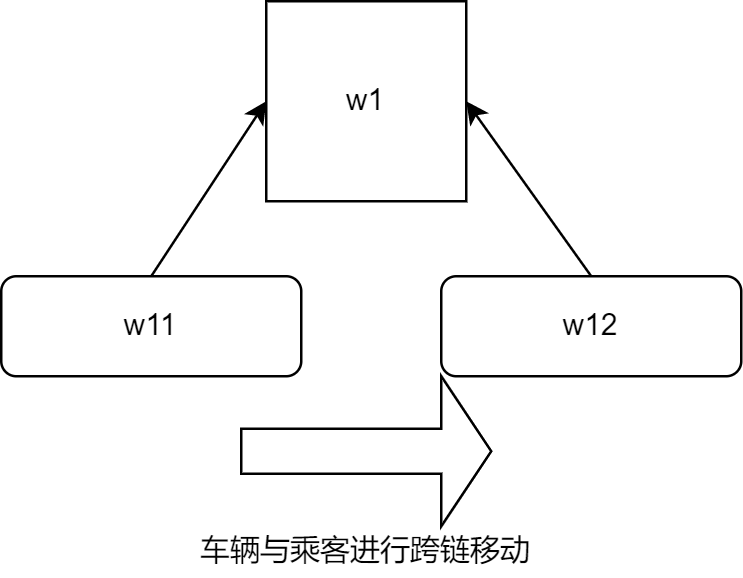
\includegraphics[width=0.5\textwidth]{figures/车辆与乘客跨链移动.png}
	\caption{车辆与乘客跨链移动}
	\label{fig:车辆与乘客跨链移动}
\end{figure}

构建一条主链记为w1,其下有两条子链分别记为w11和w12,表示的实际意义是,w1管辖Geohash编码前缀为w1的区域,w11和w12分别管辖Geohash编码前缀为w11的区域和w12的区域。此时,构建对应的区块链网络之后,在w11、w12的两条链中初始化相同的账户,各包含三个预分配账户以及10个普通账户,实验设计对于w11链中的普通账户,初始均分配有10000单位的初始资产,w12链中的普通账户,则初始资产均为0;希望模拟在账户位置进行从w11到w12的移动时,所进行的资产转移实验。具体操作为,开始实验后,树状区块链串行遍历w11中的普通账户,并发起上述的4个转账事件,将其资产转入w12链中。记录整个转账过程开始和结束的时间戳。

待试验完成之后,检查两条链中账户的资产情况便可验证,跨链转账实验的可行性,同时根据输出的时间戳来分析其性能表现。

\section{具体实验步骤}

具体的实验代码以及实验操作说明文档已存入我的毕设仓库,本小节只是简单说明一下大致流程。

\begin{enumerate}
    \item 构建上述的树状区块链网络结构,按照实验操作说明文档执行相应脚本文件即可。
    \item 依次启动两个子链开始挖矿。
    \item 由于本次实验要测试多个账户的跨链转账,且上述的转账事件有着严格的先后顺序,因此,为维护转账事件的次序性,另启动一个终端,运行branchnode-remastered.js脚本。该脚本监视父链w1的输出日志,并根据日志信息,向区块链发送交易事件,可以很好的维护转账事件的次序性。
    \item 运行脚本\verb|node transfer_test_step1.js|向w11链中的普通账户添加10000的初始金额,等待脚本运行完毕,验证w11链上的账户金额,可以发现初始金额设定成功
    \item 确认金额后,运行脚本\verb|node transfer_test_step2.js|,此时便开始了转账实验,终端中也不断发出各种转账事件的输出信息,等待转账事件全部发送完毕后,停止挖矿,实验完毕。
    \item 此时验证w11与w12中账户的资产信息。
    \item 执行\verb|node query_transfer_time.js|,脚本将访问链 w11 和链 w12 上
    的所有区块,统计其中包含的交易及其详细信息,生成测试结果报告。
\end{enumerate}

\section{测试结果分析 }

\subsection{实验正确性}

实验结果显示,原链w11中各账户的余额均为0,而链w12中的对应账户余额为10000 单位,证明了跨子链转账功能的正确性。

\subsection{性能展示}

本小节测试了10个账户的自身跨子链资产转移的测试,并分别记录了账户的转账耗时,从账户发起转账请求时开始记录,到账户资金转入目标链后结束。实验结果如图\ref{fig:账户跨子链资产转移所消耗的时间}所示:

\begin{figure}
	\centering
	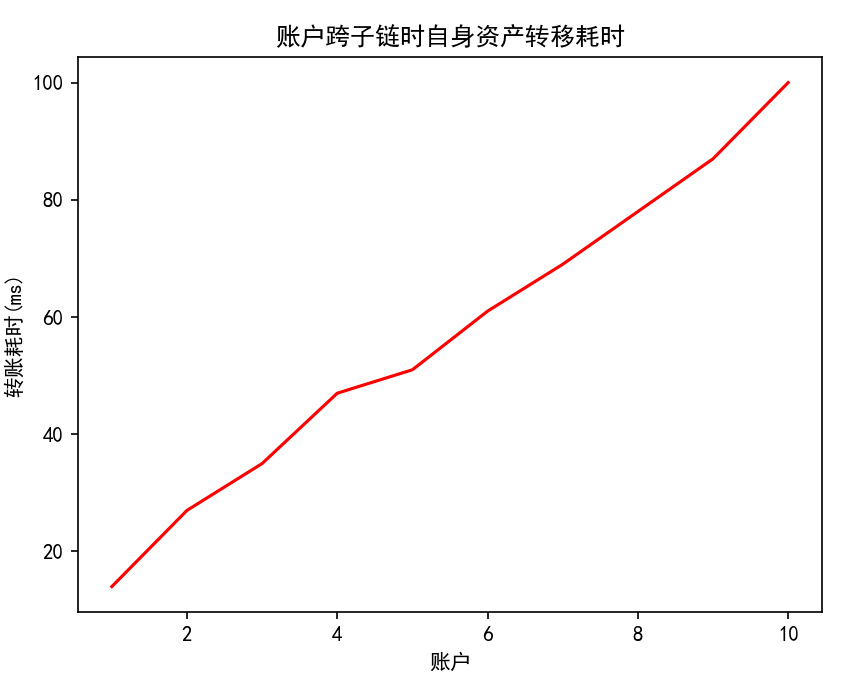
\includegraphics[width=0.8\textwidth]{figures/账户跨子链资产转移所消耗的时间.png}
	\caption{账户跨子链资产转移所消耗的时间}
	\label{fig:账户跨子链资产转移所消耗的时间}
\end{figure}

根据实验结果可以看出,账户所消耗的时间与账户的数目大致呈线性正相关。产生此现象的原因其实也并不难理解,从原理实现的角度来看,树状区块链的分支区块在处理跨链资产转移请求时,需要串行的处理并验证转账过程中相互通信的交易信息,由于跨链资产转移操作的通信过程所发送的交易信息有着严格的先后顺序,因此整个过程对外可以大致认为是一个原子性操作,耗时与账户数目线性正相关。

\section{本章小结}

本章主要介绍了树状区块链的跨链的资产转移功能。首先,阐述了实验的设计思路;之后,结合源码分析了其具体的实现过程,本章还介绍了跨链资产转移的过程中的事件函数。基于此,本章设计了账户的跨链资产转移实验,并经实验得出结论,账户跨子链进行资产转移所消耗的时间与账户的数目之间的关系大致呈线性正相关。


% !TeX root = ../thuthesis-example.tex

\chapter{实现初步的出租车调度系统的跨区域交易}

\section{实验说明}

在之前第四章的实验中,我们做了现有的基于区域搜索的树状区块链中的一条虚拟父链之下的多个子链内部的并行调度操作,验证了树状区块链在每条单链中运行出租车调度系统的可行性,并且测试了树状多链区块链的性能。但是,在之前的测试中,相互匹配的乘客与车辆账户均处于树状区块链的同一条子链当中,所有的搜索,导航,以及付款交易的操作均是在一条子链中完成;事实上这并不符合实际应用场景,因此,本章的内容主要就是围绕如何实现出租车调度系统的跨区域(跨子链)交易来展开。在本章中,我给出了跨区域交易的较为完整的逻辑架构,但是由于时间有限,我重点完成了跨子链转账的实现,将转账过程通过合约的事件交互实现,并将整个过程封装进一个函数,提供接口,使其整体形成一个原子操作,同时还实现了资产回流的操作,验证乘客是否确认上车,若成功上车则继续订单,若没成功上车,则触发资产回流;此外,我还修改了测试脚本的逻辑架构,使其更符合实际的应用情景,有关跨链搜索以及账户跨链后的资产转移部分目前完成的不够完善,仅服务于测试实验,后续若有时间,我也愿意接着进行后续的跨链交易的研究。

\section{出租车调度流程介绍}

基于现有的出租车调度系统,为了实现不同子链之间的跨链交易,我们主要需要修改的部分主要有四点:

\begin{enumerate}
    \item 整体测试代码的逻辑架构
    \item 车辆选择的过程
    \item 乘客账户向车辆账户支付订单的过程(即跨链转账)
    \item 乘客账户及车辆账户随位置改变而进行账户资产转移的过程
\end{enumerate}

如图\ref{fig:出租车调度系统的跨区域交易运行流程图}所示,相较于第四章中较为简单的调度过程,跨链的出租车调度系统的逻辑过程更加复杂。

\begin{figure}
	\centering
	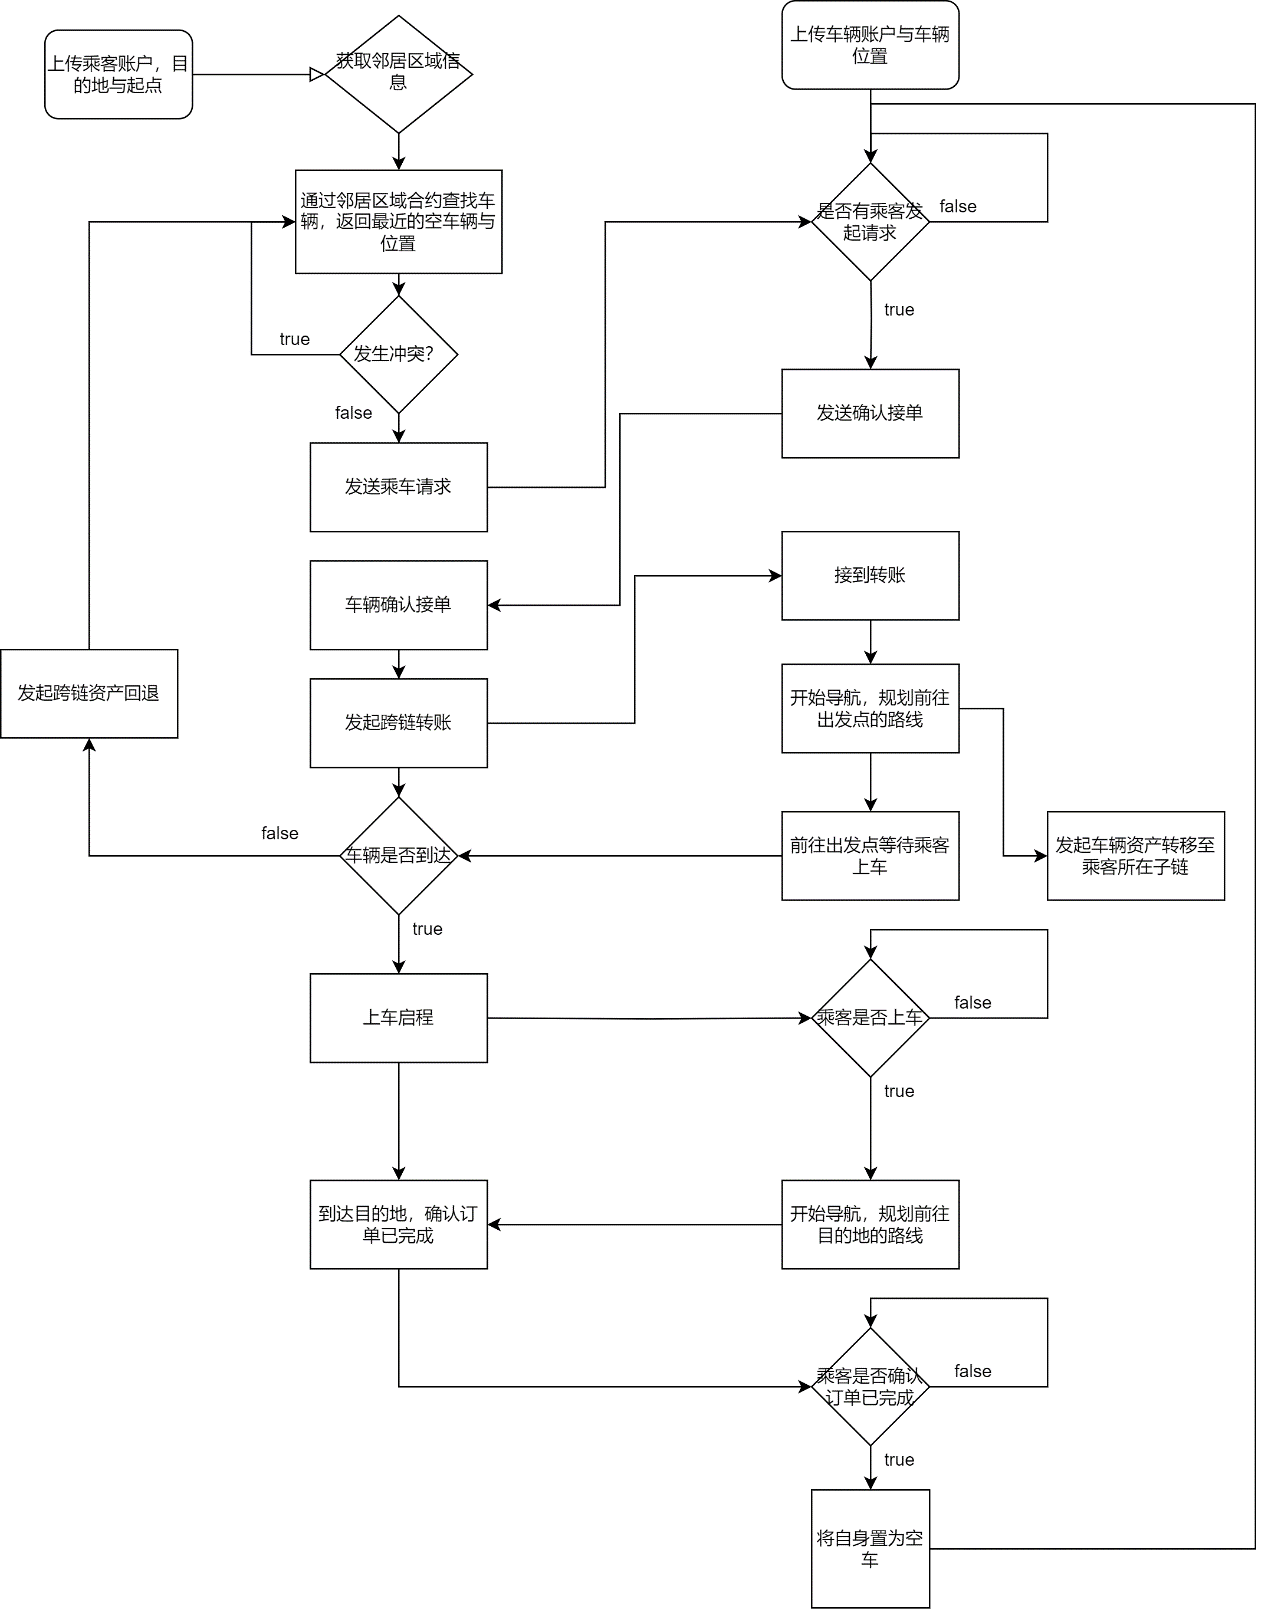
\includegraphics[width=\textwidth]{figures/出租车调度系统的跨链交易运行流程图.png}
	\caption{出租车调度系统的跨区域交易运行流程图}
	\label{fig:出租车调度系统的跨区域交易运行流程图}
\end{figure}

对于乘客端而言其操作流程大致为:

\begin{enumerate}
    \item 上传起点与目的地
    \item 获取邻居信息,初始设定搜索半径r,判断初始起点位置周围的半径的r圆是否进入了别的邻居区域,若不进入,则仍是简单的单子链内的操作;若进入,则通过父链获取邻居的合约地址,按顺序调用合约的getVehicle函数,汇总结果,得到最近的车辆及其账户,判断此交易是否需要跨链(若不跨链则仍是单子链内操作,本章内容主要考虑需要跨链的情况下的处理,因此,接下来的描述中默认匹配到的车辆需要跨链操作)。
    \item 选择车辆等待确认(这一步触发异步机制,同时只有同一个乘客可以选择一个车辆),在车辆确认接单后,发起跨链的转账。
    \item 跨链转账完成后,还需要考虑交易终止的资产回退问题,若车辆未能到达,乘客未能上车,则会触发跨链的资产回退
    \item 乘客上车启程之后,等待到达目的地时向车辆发送一个确认订单结束。
\end{enumerate}

对于车辆端而言其操作流程大致为:

\begin{enumerate}
    \item 上传起点与目的地
    \item 有乘客请求之后,向乘客发送确认接单
    \item 在跨链转账完成后,开始导航并规划前往乘客出发点的路线
    \item 注意车辆在运动到乘客所在子链区域之后,需要触发车辆的跨链资产转移
    \item 等待乘客上车后,开始导航并规划前往乘客目的地的路线
    \item 收到乘客的订单确认信息后,结束订单,将车辆状态置为空车
\end{enumerate}


\section{完成跨地区之间的车辆搜索}

\subsection{实验思路和具体实现}

本小节主要实现上述过程中的跨区域的车辆搜索问题,在本次实验中,实验规模仅仅涉及3个相邻区块,因此初始在终端中直接记录了相关的合约地址进行调用。

具体实现大致为:获取邻居信息,初始设定搜索半径r,判断初始起点位置周围的半径的r圆是否进入了别的邻居区域(此处默认搜索范围进入了相邻区块中),通过邻居的合约地址,按顺序调用合约的getVehicle函数,汇总结果,得到最近的车辆及其账户。选择车辆等待确认(这一步触发异步机制,同时只有同一个乘客可以选择一个车辆),若车辆已被占用,则等待一段时间后再次重复上述步骤。

其中,对于智能合约的修改是修改了原有的getVehicle。原本的单链程序中搜索车辆的过程是,首先获取本链中的所有车辆账户,并以此根据geohash编码计算曼哈顿距离筛选出离乘客最近的车辆,这在实际应用中是不合法的行为,修改了getVehicle,使得整个搜索过程都封装在了合约中进行,乘客能做的便是调用该合约函数,并得到返回的车辆账户的账户以及位置信息。

整体实验仓库基于第4章的实验进行,实验在真实世界地图中 Geohash 编码前缀为wx4e的区域下进行。树状区块链部分的实验在该区域下的细分区域 wx4en、wx4ep、wx4eq和wx4er区域下进行。

由于本节主要测试跨链搜索的实现的正确性,故主要选取了wx4en、wx4ep、wx4eq三条子链,其中在wx4en中初始部署乘客账户,在wx4ep、wx4eq中部署车辆账户,运行修改后的测试脚本,测试跨链搜索的实现是否正确。

在本小节的实验中,仅仅测试了跨链的车辆搜索的过程,之后的跨链转账以及车辆资产转移并未修改。具体的实验代码以及实验操作说明文档已存入本人的毕设仓库。

\subsection{实验测试}

如图在wx4en区域设立了两个乘客,并不设置车辆账户,分别在wx4ep、wx4eq中各设立一个车辆账户,基本测试数据还是用第4章中的点位数据

实验将表\ref{测试数据位点}中所示之点位,作为本章测试的测试数据位点。

\begin{table}
    \centering
    \caption{测试数据位点}\label{测试数据位点}
    \begin{tabular}{cccc} \toprule
        区域Geohash前缀 & 乘客起点        & 乘客终点        & 司机初始位置      \\\hline
        wx4en       & wx4enscgue5 & wx4enrq9mm9 & wx4enrq9mm9 \\
        wx4ep       & wx4epb8scg1 & wx4ep8e5gw0 & wx4ep8e5gw0 \\
        wx4eq       & wx4eq7rgmxk & wx4eqt6u0vu & wx4eqt6u0vu \\
        \bottomrule
    \end{tabular}
\end{table}

实验具体流程如仓库所示:

\begin{enumerate}
    \item 准备测试用的司乘数据,结果存于仓库中的json格式的文件中。
    \item 按照操作顺序启动三条子链,构建三子链网络,确保初始账号相同,且账号解锁。
    \item 在三子链上分别部署合约,并在乘客端和司机端的测试脚本中更新合约地址。
    \item 上传地图文件。
    \item 依次启动三条子链开始挖矿,同时运行乘客端和司机端的测试脚本,等待测试结束。
    \item 根据输出日志判断,跨链搜索实验是否成功。
\end{enumerate}

\subsection{实验结果}

在搜索过程中,车辆端的实验日志输出如下,具体参见仓库中的实验截图:

\begin{verbatim}

accountAddr:0xdedee68f2020c0d3f98d2a8c23b6563f7b97e559
车辆正在上传位置
车辆账户加入:0xdedee68f2020c0d3f98d2a8c23b6563f7b97e559
wx4ep8e5gw0第1辆车加入
Myevent:Myevent_vehicleId: 
0xdedee68f2020c0d3f98d2a8c23b6563f7b97e559000000000000
000000000000
Send_Confirm:0xdedee68f2020c0d3f98d2a8c23b6563f7b97e559
Beginevent:Beginevent_vehicleId: 0xdedee68f2020c0d3f98d
2a8c23b6563f7b97e559000000000000000000000000
0xdedee68f2020c0d3f98d2a8c23b6563f7b97e559接到了乘客 
0x12d0e4381ef94a70a49252e35b9a65fadd3872b90000000000000
00000000000 的订单, 乘客位置:  wx4epb8scg1

\end{verbatim}

实验结果显示,本小节实现的跨链搜索可以正确运行。

\section{实现跨区域的交易转账}

\subsection{实验思路和具体实现}

本小节也是本章的重点,主要实现的是如图\ref{fig:出租车调度系统的跨区域交易运行流程图}中跨链转账的部分。在实际应用场景当中,预付款或者提前支付定金是十分必要的,在此前的树状区块链出租车调度系统当中,仅仅支持同一条子链内部的转账操作,且其是在乘客确认订单完成后,才会发起转账支付。虽然在车辆进入到乘客所在的子链区域范围后,通过车辆账户的自身跨链资产转移可以满足乘客与车辆进行交易的条件,但是实际应用场景中,提前支付或者支付定金是对司机权益的一种保障,否则如果乘客中途退单,司机就会有空车返回的风险。本小节的主要实现目标便是希望树状区块链的出租车调度系统也可以满足跨链的提前支付。

本小节内容主要基于第五章《基于树状区块链的跨链转账测试》来做。在第五章中已经介绍过,一个账户在跨区域时需要将账户金额转移至目标区域的子链的这一过程,我根据此操作并结合源码,测试并验证出了跨链转账的可行性,我将此功能封装进了一个函数,并给出了一个具有较高鲁棒性且便于调用的函数接口,我将其放入了文章附录中,在上述的6.3小节的实验基础上,测试并实验不同地区账户之间的转账操作。

在本小节的实验中,我在跨链搜索车辆的基础上测试了之后的跨链转账过程,后续的车辆资产转移部分并未修改,故最终验证结果时,也还是在车辆的原有链中验证车辆账户余额。

\subsection{跨链转账的过程}

如图\ref{fig:出租车调度系统的跨链转账示意图}所示,跨链转账的过程:

\begin{figure}
	\centering
	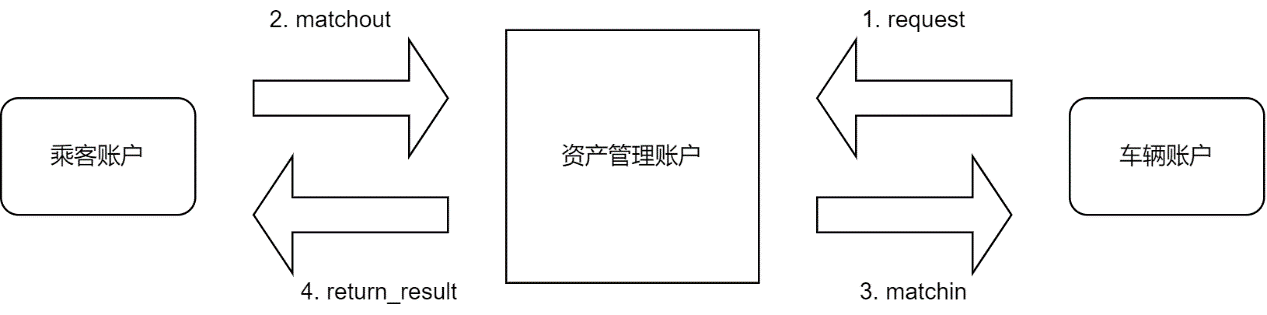
\includegraphics[width=\textwidth]{figures/出租车调度系统的跨链转账示意图.png}
	\caption{出租车调度系统的跨链转账示意图}
	\label{fig:出租车调度系统的跨链转账示意图}
\end{figure}

调用附录中实现的跨子链资产转移函数,首先是车辆账户需要向父链的资产管理账户发送一个request请求,记录request请求产生的hash值,之后乘客端会向父链的资产管理账户发送一个matchout转账请求,记录matchout请求产生的hash值。接着,父链的资产管理账户会向车辆端发送一个matchin转账请求,经过对于源码的研究,这一步操作分支区块会将此matchin与request请求进行匹配,注意对应的交易hash值也应匹配。上述工作均完成后,父链的资产管理账户会向乘客端发送一个return-result请求,记录并验证交易结果。

\subsection{实验测试}

本小节的实验基于第六章第3小节中的实验来做,实验数据选取的是,6.3小节中的实验数据。具体操作流程以及代码修改详见本人的毕设仓库。

实验具体流程见仓库,大致流程如下:

\begin{enumerate}
    \item 准备测试用的司乘数据,结果存于仓库中的json格式的文件中。
    \item 按照操作顺序启动三条子链,构建三子链网络,确保初始账号相同,且账号解锁。
    \item 在三子链上分别部署合约,并在乘客端和司机端的测试脚本中更新合约地址。
    \item 上传地图文件
    \item 依次启动三条子链开始挖矿,同时运行乘客端和司机端的测试脚本,等待测试结束。
    \item 根据输出日志验证跨链转账交易流程的正确性。
    \item 在命令行查验车辆账户余额,对比车辆账户金额验证跨链转账交易是否成功。
\end{enumerate}

\subsection{实验结果}

在实验过程中,乘客端的实验日志输出如下,具体可详见仓库中的实验截图(包含日志输出截图以及账户余额截图)

\begin{verbatim}

开始支付订单
vel 0xdedee68f2020c0d3f98d2a8c23b6563f7b97e559
res: 0xa683e5d4982e63a9b4babbab21aad1090c673806ad98ba98
dfab582bedd368e3
hash_request: 0x307861363833653564343938326536336139623
4626162626162323161616431303930633637333830366164393862
61393864666162353832626564643336386533
get_outchain_info--outchain_balance: 100000000000000
Result: 0x7e61314b0e7b5ae7c229cebfc71657bebf9cd48eda
ae0702933bd9471af19bd7
乘客支付了订单
send_inchain--Result: 0xc27f230d538a429049565caf52b63d3
f2bbc3605558d4d630ec0cad0c95c3dca
send_inchain--hash_in: 0x307863323766323330643533386134
3239303439353635636166353262363364336632626263333630353
53538643464363330656330636164306339356333646361
send_inchain--balance: 100000000000000
send_result--Tx_result: 0x78be78c00f0aae68e2e93fdc1676b
bc78d0eacf82b994ab1b891dfd1c6de9b1c
乘客确认交易结束

\end{verbatim}

表明本小节实现的跨链转账交易可以正确运行。经过在命令行查看车辆账户余额,可以看到:

如表\ref{实验账户公钥}中所示,分配实验账户:

\begin{table}
    \linespread{1.5}
    \centering
    \caption{实验账户公钥}\label{实验账户公钥}
    \begin{tabular}{cc} \toprule
        乘客车辆账户                  & 公钥地址                         \\ \hline
        Wx4ep链中的车辆账户acc1 & 0xdedee68f2020c0d3f98d2a8c23b6563f7b97e559            \\
        Wx4eq链中的车辆账户acc2   & 0xad8a321e2e8f8f51245f47b8f412979d5740e625            \\
        Wx4en链中的乘客账户acc3   & 0x12d0e4381ef94a70a49252e35b9a65fadd3872b9 
        \\
        Wx4en链中的乘客账户acc4   & 0x456c4df0610c7611ae8bcaed32dd1d94e88ceca4
        \\\bottomrule
    \end{tabular}
\end{table}

账户初始金额:50000000000000000000
如表\ref{实验结果}所示:

\begin{table}
    \linespread{1.5}
    \centering
    \caption{实验结果}\label{实验结果}
    \begin{tabular}{ccc} \toprule
        账户类别                & 账户                 & 转账实验后金额            \\ \hline
        Wx4ep链中的车辆账户 & acc1   & 50000892848000000000                \\
        Wx4eq链中的车辆账户 & acc2   & 50000892848000000000                \\
        Wx4en链中的乘客账户 & acc3   & 49998851463000000000 
        \\
        Wx4en链中的乘客账户 & acc4   & 49998866463000000000
        \\\bottomrule
    \end{tabular}
\end{table}

结果显示,车辆账户收到转账,验证了本节实现的跨链转账的正确性。
注意到本区块链中两个账户使用相同的合约函数发送相同的请求,send中设定的gas值也一样,但最终消耗的gas值不一样,推测这可能是因为第一次调用该函数会触发合约代码的初始化,需要加载更多的资源和执行更多的操作,因此会消耗更多的gas。而后续的调用由于已经完成了初始化,所以消耗的gas会稳定在一个较小的范围内。

\section{跨区域交易合约}

\subsection{实验思路和具体实现}

将上述测试脚本的运行逻辑进行改进,使得整个过程都是基于合约中的事件来触发,修改了原有的traffic合约,并新实现了一个transfer合约用于跨链转账的过程中进行通信交互,使得整体过程更趋于实际的应用过程。并且将该过程由合约封装后,在实际的高负载应用中可以维护跨链转账交易的原子性;同时,实际转账操作也对用户隐藏,对外仅提供完成转账操作的合约函数接口。

同样如图\ref{fig:出租车调度系统的跨链转账示意图}所示,具体的合约封装的转账流程如下:

\begin{enumerate}
    \item 首先是车辆账户需要向父链的资产管理账户发送一个request请求,同时,通过合约函数发送交易双方的账户,以及request请求产生的hash值。
    \item 乘客端接收到该事件后,乘客端会向父链的资产管理账户发送一个matchout转账请求,同时,乘客端通过合约函数发送交易双方的账户转账金额,以及matchout请求产生的hash值。
    \item 车辆端接收到该事件后,父链的资产管理账户会向车辆端发送一个matchin转账请求,经过对于源码的研究,这一步操作分支区块会将此matchin与request请求进行匹配,同时,通过合约函数发送交易双方的账户转账金额,以及matchin请求产生的hash值。
    \item 乘客端接收到该事件后,表明此时matchout和matchin请求都已成功,父链的资产管理账户会向乘客端发送一个return-result请求,记录并验证交易结果。
\end{enumerate}

这里以matchout为例,大致展现一下算法操作。
% \subsection{算法}

% 算法环境可以使用 \pkg{algorithms} 或者 \pkg{algorithm2e} 宏包。

\renewcommand{\algorithmicrequire}{\textbf{输入:}\unskip}
\renewcommand{\algorithmicensure}{\textbf{输出:}\unskip}

\begin{algorithm}
  \linespread{1.5}
  \caption{send—matchout}
  \label{alg1}
  \small
  \begin{algorithmic}
    \REQUIRE $from$$-$$address$ $ $
    $to$$-$$address$  $ $
    $web$  $ $
    $value$ 

    \STATE $web.events.In$$-$$Event1$
        \IF{$event.passengerId$ is $from$$-$$address$ and 
        $event.vehicleId$ is $to$$-$$address$ }
            \STATE $sendTransaction(Matchout)$
            \STATE $console.log(Matchout)$
        \ENDIF
      
  \end{algorithmic}
\end{algorithm}

\subsection{实验测试}

本小节的实验基于第六章第4小节中的实验来做,本小节实验需要验证跨链转账操作的原子性,故引入单链中的冲突事件,初始设定10个账户参与测试(4个车辆账户,wx4ep区域中2个,wx4eq区域中2个;6个乘客账户,均位于wx4en区域中),实验的位点数据选取的仍是,6.4小节中的实验数据。具体操作流程以及代码修改详见本人的毕设仓库。

如表\ref{多账户实验账户公钥}中所示,分配实验账户:

\begin{table}
    \linespread{1.5}
    \centering
    \caption{多账户实验账户公钥}\label{多账户实验账户公钥}
    \begin{tabular}{cc} \toprule
        乘客车辆账户                  & 公钥地址                                           \\ \hline
Wx4ep链中的车辆账户acc1 & 0x7a68b86008b0cfc3ae0e8068360271cbb999c97d
        \\
Wx4ep链中的车辆账户acc2   & 0xd5f5ef5ff4c6323c62bdc5ab2061f440aefc511b    
        \\
Wx4eq链中的车辆账户acc3   & 0xd402c7301a68c4c65529ab0c597bb8b13e27f607
        \\
Wx4eq链中的车辆账户acc4   & 0x42389309e69a2b32b98f04bc8255ad971797f757
        \\
Wx4en链中的乘客账户acc5  & 0xdedee68f2020c0d3f98d2a8c23b6563f7b97e559
        \\
Wx4en链中的乘客账户acc6   & 0xc0a3917e5679c0ef9033c41cbe294a212abe55df             \\
Wx4en链中的乘客账户acc7   & 0x55577fd620a0b8379846fcb1499e4bdc22538843
        \\
Wx4en链中的乘客账户acc8   & 0xad8a321e2e8f8f51245f47b8f412979d5740e625
        \\
Wx4en链中的乘客账户acc9  & 0x91153bad44dcc46187c481d8d36a53e58522d0c4
        \\
Wx4en链中的乘客账户acc10   & 0xe64e81bc77ee05caaa6b1476de75193607e84d87                             
        \\\bottomrule
    \end{tabular}
\end{table}


\subsection{实验结果}

在实验过程中,实验日志输出如下,具体可详见仓库中的实验截图(包含日志输出截图以及账户余额截图):

\begin{verbatim}
    IN_transf1
    IN_Event1
    send_inchain--Result: 0xc27f230d538a429049565caf52b
    63d3f2bbc3605558d4d630ec0cad0c95c3dca
    send_inchain--hash_in: 0x30786332376632333064353338
    613432393034393536356361663532623633643366326262633
    336303535353864346436333065633063616430633935633364
    6361
    send_inchain--balance: 100000000000000
    send_result--Tx_result: 0x78be78c00f0aae68e2e93fdc1
    676bbc78d0eacf82b994ab1b891dfd1c6de9b1c
    OUT_Event2
    send_result--Tx_result: end
    IN_Event3
    RE_Event4
\end{verbatim}

日志中输出了合约函数的事件触发信息,表明本小节实现的跨链转账交易的合约封装可以正确运行。经过在命令行查看车辆账户余额,可以看到:


账户初始金额:50000000000000000000,实验结果
如表\ref{Wx4ep链中的车辆账户}、\ref{Wx4eq链中的车辆账户}、\ref{Wx4en链中的乘客账户}所示:

\begin{table}
    \linespread{1.5}
    \centering
    \caption{Wx4ep链中的车辆账户}\label{Wx4ep链中的车辆账户}
    \begin{tabular}{*{3}{>{\centering\arraybackslash}p{4cm}}} \toprule
        账户                & 转账实验后金额            \\ \hline
        acc1   & 50000907848000000000               \\
        acc2   & 50001892848000000000              \\
        \bottomrule
    \end{tabular}
\end{table}


\begin{table}
  \linespread{1.5}
  \centering
  \caption{Wx4eq链中的车辆账户}
  \begin{tabular}{*{2}{>{\centering\arraybackslash}p{4cm}}}
    \toprule
    账户                & 转账实验后金额         \\
    \midrule
    acc3   & 50000907848000000000               \\
    acc4   & 50001892848000000000               \\
    \bottomrule
  \end{tabular}
  \label{Wx4eq链中的车辆账户}
\end{table}


\begin{table}
    \linespread{1.5}
    \centering
    \caption{Wx4en链中的乘客账户}\label{Wx4en链中的乘客账户}
    \begin{tabular}{*{2}{>{\centering\arraybackslash}p{4cm}}} \toprule
        账户                & 转账实验后金额           \\ \hline
        acc5   & 49998851463000000000               \\
        acc6   & 49998866463000000000               \\
        acc7   & 49998866463000000000               \\
        acc8   & 49998866463000000000               \\
        acc9   & 49998866463000000000               \\
        acc10   & 49998866463000000000              \\
        \bottomrule
    \end{tabular}
\end{table}

可以看出车辆账户金额增多,转账实验验证成功。同时,转账事件之间并无冲突,验证了跨链转账操作的原子性实现的正确性。

\section{实验不足性说明}

\subsection{搜索方面的简化}

在搜索车辆时,需要获取邻居子链的合约的地址信息,这部分操作需要与父链相结合来完成,目前并未完整的实现与父链进行交互的这一搜索过程。而是为了简化验证跨链搜索的正确性直接在终端部署了邻居子链的合约地址。

\subsection{车辆运行的简化}

在实际的应用程序中,应该要能够实时展示乘客与车辆的位置信息,并且要及时将位置信息上传到区块链当中,此部分目前并未与前端相结合实现,由于本章重点验证的跨链交易的实现,故在测试脚本代码中省略了车辆调度过程中时时上传地理位置信息的操作。

\subsection{资产转移的省略}

在车辆跨链进入乘客所在的子链时,需要触发车辆账户的资产转移,本事件并未在本章节中体现,不过,跨链资产转移的实现以及相关测试第五章中均已完成,故后续在本章节中添加资产转移的事件也是较为容易的,在此简单叙述一下实现的逻辑过程:在车辆实时上传地理位置信息的操作前添加对于位置信息的判断,若超出了当前所处链的范围,则需触发跨链的资产转移。

\section{本章小结}

本章的内容主要就是围绕如何实现出租车调度系统的跨链交易来展开。在本章中,我给出了跨链交易的较为完整的逻辑架构,同时完成了其中的跨链转账的实现,将转账过程通过合约的事件交互实现,并将整个过程封装进一个函数,提供接口,使其整体形成一个原子操作,同时还实现了资产回流的操作,验证乘客是否确认上车,若成功上车则继续订单,若没成功上车,则触发资产回流;此外,我还修改了测试脚本的逻辑架构,使其更符合实际的应用情景。

目前实验的不足在于有关跨区域搜索以及账户跨区域后的资产转移部分目前完成的尚不够完善,仅服务于测试实验。我给出了其实际应用情形的逻辑架构,便于后续研究者的研究与实现,后续若有时间,我们将继续开展后续的跨区域交易的研究。


% !TeX root = ../thuthesis-example.tex

\chapter{结论}

% \begin{conclusion}
将区块链技术应用于车联网中,可以实现司乘之间的可信交流,降低信任成本,有利于安全高效的交通体系的构建。然而,传统区块链的单链结构,在处理大量交易时,执行效率无法得到保证。为解决该问题,实验室提出在出租车调度系统中应用“树状区块链”,以满足更加复杂以及更加贴合实际应用的调度需求。在现有的基于树状区块链实现的出租车调度系统中,司乘之间的匹配与交易仅能在同一子链所在的地理区域内完成,在实际应用中有着较为明显的局限性。
  
本文首先完成了对于实现区域搜索的树状区块链的前期调研,理解了其在出租车调度系统中的工作过程。

其次,本文完成了对于在出租车调度系统中应用树状区块链的实验复现,并完善了实验手册。

之后,本文做了树状多链区块链应用到出租车调度系统上的性能测试实验。通过javascript脚本来模拟乘客端与车辆端的交互行为;在四条子链上并行运行调度系统,将其与单链的平均性能进行对比,分析数据并得出结论。

接着,本文介绍了树状区块链的一个账户的跨子链资产转移功能,介绍了此功能的作用场景,并结合源码实现分析了其工作原理。此外,本文针对此功能还设计了验证实验,验证了该操作的原子性,并测试了其性能效率。

最后,本文尝试对现有的出租车调度系统进行改进,实现树状区块链的跨链的交易操作,并最终给出了一个简易的能够实现跨链交易的调度过程,使出租车调度系统能满足不同区域间的账户交易。并设计实验验证了实现的正确性。

整体而言,本文工作较好的完成了跨链转账的过程的合约封装,通过完善原有的单链出租车调度系统的逻辑,使其初步满足了跨链之间的出租车调度,丰富了原有调度系统的功能,使其更加切合现实应用。但本文工作目前来看仍有较大的可扩展空间,比如,可以改进搜索算法,使得车辆匹配的过程更快;可以添加实时路径,还有车乘共同跨链的情况需要考虑等。

% \end{conclusion}
% 其他部分
\backmatter

% 插图和附表清单
% 本科生的插图索引和表格索引需要移至正文之后、参考文献前
% \listoffiguresandtables  % 插图和附表清单(仅限研究生)
\listoffigures           % 插图清单
\listoftables            % 附表清单

% 参考文献
\bibliography{ref/refs}  % 参考文献使用 BibTeX 编译
% \printbibliography       % 参考文献使用 BibLaTeX 编译

% 声明
% \statement
% 将签字扫描后的声明文件 scan-statement.pdf 替换原始页面
% \statement[file=scan-statement.pdf]
% 本科生编译生成的声明页默认不加页脚,插入扫描版时再补上;
% 研究生编译生成时有页眉页脚,插入扫描版时不再重复。
% 也可以手动控制是否加页眉页脚
% \statement[page-style=empty]
\statement[file=scan-statement.pdf, page-style=plain]
\statement[file=声明.pdf, page-style=plain]

% 附录
% 本科生需要将附录放到声明之后,个人简历之前
\appendix
% % !TeX root = ../thuthesis-example.tex

\begin{survey}
\label{cha:survey}

\title{Title of the Survey}
\maketitle


\tableofcontents


本科生的外文资料调研阅读报告。


\section{Figures and Tables}

\subsection{Figures}

An example figure in appendix (Figure~\ref{fig:appendix-survey-figure}).

\begin{figure}
  \centering
  
\includegraphics[width=0.6\linewidth]{example-image-a.pdf}
  \caption{Example figure in appendix}
  \label{fig:appendix-survey-figure}
\end{figure}


\subsection{Tables}

An example table in appendix (Table~\ref{tab:appendix-survey-table}).

\begin{table}
  \centering
  \caption{Example table in appendix}
  \begin{tabular}{ll}
    \toprule
    File name       & Description                                         \\
    \midrule
    thuthesis.dtx   & The source file including documentaion and comments \\
    thuthesis.cls   & The template file                                   \\
    thuthesis-*.bst & BibTeX styles                                       \\
    thuthesis-*.bbx & BibLaTeX styles for bibliographies                  \\
    thuthesis-*.cbx & BibLaTeX styles for citations                       \\
    \bottomrule
  \end{tabular}
  \label{tab:appendix-survey-table}
\end{table}


\section{Equations}

An example equation in appendix (Equation~\eqref{eq:appendix-survey-equation}).
\begin{equation}
  \frac{1}{2 \uppi \symup{i}} \int_\gamma f = \sum_{k=1}^m n(\gamma; a_k) \mathscr{R}(f; a_k)
  \label{eq:appendix-survey-equation}
\end{equation}


\section{Citations}

Example citations in appendix.
\cite{abrahams99tex}
\cite{salomon1995advanced}
\cite{abrahams99tex,salomon1995advanced}


\bibliographystyle{unsrtnat}
\bibliography{ref/appendix}

\end{survey}
       % 本科生:外文资料的调研阅读报告
% !TeX root = ../thuthesis-example.tex

\begin{translation}
\label{cha:translation}

\title{书面翻译题目}
\maketitle

\tableofcontents


本科生的外文资料书面翻译。


\section{图表示例}

\subsection{图}

附录中的图片示例(图~\ref{fig:appendix-translation-figure})。

\begin{figure}
  \centering
  
\includegraphics[width=0.6\linewidth]{example-image-a.pdf}
  \caption{附录中的图片示例}
  \label{fig:appendix-translation-figure}
\end{figure}


\subsection{表格}

附录中的表格示例(表~\ref{tab:appendix-translation-table})。

\begin{table}
  \centering
  \caption{附录中的表格示例}
  \begin{tabular}{ll}
    \toprule
    文件名          & 描述                         \\
    \midrule
    thuthesis.dtx   & 模板的源文件,包括文档和注释 \\
    thuthesis.cls   & 模板文件                     \\
    thuthesis-*.bst & BibTeX 参考文献表样式文件    \\
    thuthesis-*.bbx & BibLaTeX 参考文献表样式文件  \\
    thuthesis-*.cbx & BibLaTeX 引用样式文件        \\
    \bottomrule
  \end{tabular}
  \label{tab:appendix-translation-table}
\end{table}


\section{数学公式}

附录中的数学公式示例(公式\eqref{eq:appendix-translation-equation})。
\begin{equation}
  \frac{1}{2 \uppi \symup{i}} \int_\gamma f = \sum_{k=1}^m n(\gamma; a_k) \mathscr{R}(f; a_k)
  \label{eq:appendix-translation-equation}
\end{equation}


\section{文献引用}

文献引用示例\cite{abrahams99tex}。


\appendix

\section{附录}

附录的内容。


% 书面翻译的参考文献
\bibliographystyle{unsrtnat}
\bibliography{ref/appendix}

% 书面翻译对应的原文索引
\begin{translation-index}
  \nocite{salomon1995advanced}
  \bibliographystyle{unsrtnat}
  \bibliography{ref/appendix}
\end{translation-index}

\end{translation}
  % 本科生:外文资料的书面翻译
% !TeX root = ../thuthesis-example.tex

\chapter{补充内容}

\section{跨子链资产转移函数}

\begin{verbatim}
async function trans_tx(from_add ,to_add, web_to) {
let hashRequests = " ";
	web_to.eth.sendTransaction(
		{ from: to_add, to: accountManagerW11, position:
  POSITION1, txtype: 1, txtime: Date.now()},
		function (err, res) {
			if (err) {
				console.error("Error:", err);
			} else {
				hashRequests = web_to.utils.asciiToHex(res);
				console.log(`hash_request: ${hashRequests}`);
			}
		});

	let hash_req = hashRequests;
const macc_outbal = web3.eth.getBalance(from_add);
        
	web3.eth.sendTransaction({ from: from_add, 
 to: accountManagerW11, value: macc_outbal, 
 position: POSITION, txtype: 2, txtime:
 Date.now(), exdata: hash_req }
, function (err, res) {
		if (err) {
			console.log("Error:", err);
		} else {
			hash_out = web3.utils.asciiToHex(res);
			send_inchain_tx(web_to, to_add, macc_outbal,
   hash_out, POSITION1, web3, POSITION);
return;
		}
	});
}

async function send_inchain_tx(inweb3, acc, inbal, 
txouthash, inpos, outweb3, outpos) {
	inweb3.eth.sendTransaction({ from: accountManagerW11,
 to: acc, value: inbal, position: inpos, txtype: 3,
 txtime: Date.now(), exdata: txouthash }
, function (err, res) {
		if (err) {
			console.log("Error:", err);
		} else {
			console.log("send_inchain--Result:", res);
			hash_in = inweb3.utils.asciiToHex(res);
			console.log("send_inchain--hash_in:", hash_in);
			var macc1_inbal = inweb3.eth.getBalance(acc)
			console.log("send_inchain--balance:", macc1_inbal)
			send_result_tx(outweb3, acc, true, hash_in, outpos);
return;
		}
	});
}

function send_result_tx(outweb3, acc, result, txinhash,
outpos) {
	if (result) {
		outweb3.eth.sendTransaction({ from: accountManagerW11, 
  to: acc, position: outpos, txtype: 4,
  txtime: Date.now(), exdata: txinhash }
, function (err, res) {
			if (err) {
				console.log("Error:", err);
			} else {
				console.log("send_result--Tx_result:", res);
				endtime = new Date().getTime();
				console.log("during--", endtime - starttime)
return;
			}
		});
return;
	}
}
\end{verbatim}

\section{Github 地址索引}

本文工作对应的 Github 仓库地址为:
https://github.com/diyz19/GraduationDesign

% \printbibliography


% 致谢
% !TeX root = ../thuthesis-example.tex

\begin{acknowledgements}
  在本文完成的过程中,我受到了来自许多人的鼓励、支持和帮助。衷心感谢以下人士对我的帮助:
  
  首先我要感谢向勇老师对本人的精心指导。这段时间的毕设研究不仅仅是知识方面的学习,更是培养了我做合作研究时的一些好习惯,他的言传身教将使我终生受益。
  
  感谢课题组中周畅前辈的指导以及其他前辈们的实验手册,他们的帮助使得我可以快速入门课题,他们的研究经验对我来说也是宝贵的财富。
  
  我想感谢我的父母,是他们一直给予我鼓励与支持,让我可以继续勇敢前行。还要感谢我的三位室友,大学四年的相处让我们彼此成为了最好的伙伴,在学习和工作上他们都给了我极大的帮助。

  在此,再一次向以上所有人表示我的感谢和敬意。
\end{acknowledgements}



% 个人简历、在学期间完成的相关学术成果
% 本科生可以附个人简历,也可以不附个人简历
% % !TeX root = ../thuthesis-example.tex

\begin{resume}

  \section*{个人简历}

  197× 年 ×× 月 ×× 日出生于四川××县。

  1992 年 9 月考入××大学化学系××化学专业,1996 年 7 月本科毕业并获得理学学士学位。

  1996 年 9 月免试进入清华大学化学系攻读××化学博士至今。


  \section*{在学期间完成的相关学术成果}

  \subsection*{学术论文}

  \begin{achievements}
    \item Yang Y, Ren T L, Zhang L T, et al. Miniature microphone with silicon-based ferroelectric thin films[J]. Integrated Ferroelectrics, 2003, 52:229-235.
    \item 杨轶, 张宁欣, 任天令, 等. 硅基铁电微声学器件中薄膜残余应力的研究[J]. 中国机械工程, 2005, 16(14):1289-1291.
    \item 杨轶, 张宁欣, 任天令, 等. 集成铁电器件中的关键工艺研究[J]. 仪器仪表学报, 2003, 24(S4):192-193.
    \item Yang Y, Ren T L, Zhu Y P, et al. PMUTs for handwriting recognition. In press[J]. (已被Integrated Ferroelectrics录用)
  \end{achievements}


  \subsection*{专利}

  \begin{achievements}
    \item 任天令, 杨轶, 朱一平, 等. 硅基铁电微声学传感器畴极化区域控制和电极连接的方法: 中国, CN1602118A[P]. 2005-03-30.
    \item Ren T L, Yang Y, Zhu Y P, et al. Piezoelectric micro acoustic sensor based on ferroelectric materials: USA, No.11/215, 102[P]. (美国发明专利申请号.)
  \end{achievements}

\end{resume}


% 指导教师/指导小组评语
% 本科生不需要
% % !TeX root = ../thuthesis-example.tex

\begin{comments}
% \begin{comments}[name = {指导小组评语}]
% \begin{comments}[name = {Comments from Thesis Supervisor}]
% \begin{comments}[name = {Comments from Thesis Supervision Committee}]

  论文提出了……

\end{comments}


% 答辩委员会决议书
% 本科生不需要
% % !TeX root = ../thuthesis-example.tex

\begin{resolution}

  论文提出了……

  论文取得的主要创新性成果包括:

  1. ……

  2. ……

  3. ……

  论文工作表明作者在×××××具有×××××知识,具有××××能力,论文××××,答辩××××。

  答辩委员会表决,(×票/一致)同意通过论文答辩,并建议授予×××(姓名)×××(门类)学博士/硕士学位。

\end{resolution}


% 本科生的综合论文训练记录表(扫描版)
% \record{file=scan-record.pdf}
\record{file=综合论文训练记录表.pdf}

\end{document}
